\documentclass[a4paper]{article}
%AMDG
\usepackage{amsmath, amsthm, amssymb}
\usepackage{hyperref}
\usepackage[slovene]{babel}
\usepackage[utf8]{inputenc}
\usepackage[T1]{fontenc}
\usepackage{epigraph}
\usepackage{pdftexcmds}
\usepackage{fancyref, nameref}
\usepackage{epigraph}
\usepackage{cleveref}
\usepackage{verbatim}
\usepackage{enumitem}
\usepackage{multicol}
\usepackage[nomessages]{fp}
\usepackage{fancyhdr}
\usepackage{multirow}

\usepackage{tikz}


\parindent=0pt


% \epigraphsize{\small}% Default
\setlength\epigraphwidth{8cm}
\setlength\epigraphrule{0pt}

\usepackage{etoolbox}

\makeatletter
\patchcmd{\epigraph}{\@epitext{#1}}{\itshape\@epitext{#1}}{}{}
\makeatother


\newcounter{environment:definition_counter}

\newenvironment{definition}[1][\unskip]
{\vspace{0.5cm}\refstepcounter{environment:definition_counter}\textbf{Definicija \arabic{environment:definition_counter}: \textbf{#1}}\itshape}
{\bigskip}

\newcounter{environment:theorem_counter}

\newenvironment{theorem}[1][\unskip]
{\refstepcounter{environment:theorem_counter}\textbf{Izrek \arabic{environment:theorem_counter}:\textit{#1}} \\}
{\bigskip}

\newcounter{environment:statement_counter}

\newenvironment{statement}[1][\unskip]
{\refstepcounter{environment:statement_counter}\textbf{Trditev \arabic{environment:statement_counter}:\textit{#1}}}
{\bigskip}

\newcounter{example:example_counter}

\newenvironment{example}
{\textbf{Primer:}\\}
{\setcounter{example:example_counter}{0}}

\newenvironment{example_case}
{\refstepcounter{example:example_counter} \arabic{example:example_counter}.}
{\\}

\newenvironment{remark}
{\textbf{Opomba:}}
{}

\newenvironment{corollary}
{\underline{\textbf{Posledica:}}}
{}

%should rethink this
\newtheorem{lemma}{Lema}

\newcommand{\subscript}[2]{$#1 _ #2$}

\newcommand{\twopartdef}[4]
{
	\left\{
		\begin{array}{ll}
			#1 & \mbox{; } #2 \\
			#3 & \mbox{; } #4
		\end{array}
	\right.
}


\pagestyle{headings}
\pagestyle{fancy}
%\fancyhead[LE,RO]{\itshape \nouppercase \rightmark}
%\fancyhead[LO,RE]{\itshape \nouppercase Chapter \arabic{chapter}}


\lfoot{Skripta za Algebro 2}
\rfoot{Filip Koprivec}

\begin{document}	
\title{Skripta za algebro 2}
\author{Filip Koprivec}
\date{\today}
\maketitle

\epigraph{“If I find in myself desires which nothing in this world can satisfy, the only logical explanation is that I was made for another world.”}{--- \textup{C. S. Lewis}}
\newpage

\tableofcontents

\newpage

\begin{comment}
Start of text
\end{comment}

\section{Osnovne algebrske strukture}
\subsection{Binarne operacije}
\begin{definition}[Binarna Operacija]
\label{def:binary_operation}
(tudi dvočlena operacija) $\circ$ na množici $\mathcal{S}$ je preslikava iz $\mathcal{S} \times \mathcal{S} \  v \ \mathcal{S}$.\\ Torej $\circ : \mathcal{S} \times \mathcal{S} \ \to \ \mathcal{S}$
\end{definition}

\begin{example}
Osnovna zgleda binarnih operacij na $\mathbb{Z}$ sta:

\begin{example_case}
Seštevanje: $(n,m) \mapsto n+m$
\end{example_case}
\begin{example_case}
Množenje: $(n,m) \mapsto n \times m$
\end{example_case}

\end{example}

Skalarni produkt v $\mathbb{R}^{2}$ \textbf{ni} binarna operacija.

Vektorski produkt v $\mathbb{R}^{3}$ \textbf{je} binarna operacija.
\\\\
\begin{definition}
\label{def:asociative_operation}
Operacija $\circ$ je \textbf{asociativna}, če ustreza enačbi
\begin{equation}
\label{eq:asociative_law}
\forall x,y,z \in \mathcal{S}.\ (x \circ y) \circ z = x \circ (y \circ z)
\end{equation}

\end{definition}

Enakost \ref{eq:asociative_law} imenujemo \textbf{Zakon o asociativnosti}\\
Operacije, ki jih bomo obravnavali bodo praviloma asociativne.

\begin{definition}
\label{def:comutative_operation}
Elementa $x,y \in \mathcal{S}$ \textbf{komutirata}, če velja 
\begin{equation}
x,y \in \mathcal{S}. x \circ y = y \circ x
\end{equation}
Če za poljubna dva elementa iz $\mathcal{S}$ velja
\begin{equation}
\label{eq:comutative_law}
\forall x,y \in \mathcal{S}. x \circ y = y \circ x
\end{equation}
pravimo, da je operacija $\circ$ komutativna.
Enakost \ref{eq:comutative_law} imenujemo \textbf{Zakon o komutativnosti}

\end{definition}
\begin{remark}
Kadar je iz konteksta razvidno, o kateri operaciji govorimo, pogosto namesto "$\circ$ je komutativna rečemo tudi $\mathcal{S}$ je komutativna"
\end{remark}

\begin{example}
\begin{example_case}
Operacija + na $\mathbb{Z}$ je tako asociativna in komutativna
\end{example_case}
\begin{example_case}
Operacija * na $\mathbb{Z}$ je tako asociativna in komutativna
\end{example_case}
\begin{example_case}
Operacija - na $\mathbb{Z}$ \textbf{ni} niti asociativna niti komutativna
\end{example_case}
\begin{remark}
Na operacijo odštevanja gledamo kot na izpeljano operacijo in ne kot na samostojna operacijo, saj jo vpeljemo preko seštevanja in pojma nasprotnega elementa.
\end{remark}

\begin{example_case}
Naj bo $\mathcal{X}$ poljubna neprazna množica. Z $F(\mathcal{X})$ označimo množico vseh preslikav iz $\mathcal{X}$ v $\mathcal{X}$. Naj bosta $f, g \in \mathcal{X}$, potem je $(f,g) \mapsto f \circ g$ (kompozitum funkcij) binarna operacija na $F(\mathcal{X})$.

\begin{remark}
Operacija je asociativna, in kadar $|\mathcal{X}| \geq 2$ ni komutativna
\end{remark}
\end{example_case}
\end{example}

\begin{definition}
\label{def:identity_element}
Naj bo $\circ$ binarna operacija na na $\mathcal{S}$ in $e \in \mathcal{S}$. $e$ se imenuje \textbf{nevtralni element}, če velja 
\begin{equation}
\label{eq:identity_element}
\forall x \in \mathcal{S}. e \circ x = x \circ e = x
\end{equation}

\end{definition}

\begin{example}
\begin{example_case}
$0$ je nevtralni element za seštevanje na $\mathbb{Z}$.
\end{example_case}
\begin{example_case}
$1$ je nevtralni element za množenje na $\mathbb{Z}$.
\end{example_case}
\begin{example_case}
$id_{x}$ (identična preslikava) je nevtralni element za $F(\mathcal{X})$
\end{example_case}
\end{example}

\begin{remark}
Nevtralni element nima zagotovljenega obstoja (recimo $+$ na $\mathbb{N}$ ali $*$ na sodih celih številih).
\end{remark}

\begin{statement}
\label{st:identity_unique}
Če nevtralni element obstaja, je en sam.
\begin{proof}
\label{pr:identity_unique}
Naj bosta $f,e \in \mathcal{S}$ nevtralna elementa.
$$e = e \circ f \text{\ \ // Ker je f nevtralni element}$$
$$e \circ f = f \text{\ \ // Ker je e nevtralni element}$$
$$e = f $$
\end{proof}
\end{statement}

\begin{definition}
\label{def:left_identity}
Element $e'$ je \textbf{levi nevtralni element}, če velja:
\begin{equation}
\label{eq:left_identity_element}
\forall x \in \mathcal{S}. e' \circ x = x
\end{equation}
\end{definition}

\begin{definition}
\label{def:right_identity}
Element $e''$ je \textbf{desni nevtralni element}, če velja:
\begin{equation}
\label{eq:right_identity_element}
\forall x \in \mathcal{S}. x \circ e'' = x
\end{equation}
\end{definition}

\begin{remark}
Levih in desnih nevtralnih elementov je lahko več

\begin{example}
\begin{example_case}
$\circ : (x,y) \mapsto y$.

Vsak element je levi nevtralni element
\end{example_case}
\begin{example_case}
$0$ je desni nevtralni element za odštevanje v $\mathbb{Z}$
\end{example_case}
\end{example}
\end{remark}

\begin{statement}
\label{st:identity_left_right_both}
Naj bo za operacijo $\circ$ $e'$ levi nevtralni element, $e''$ pa desni nevtralni element. Tedaj velja $e' = e'' = e$ (Sta si levi in desni nevtralni element enaka in je(sta) nevtralni element)
\begin{proof}
\label{pr:identity_left_right_both}
$$e' = e' \circ e'' = e''$$
\end{proof}
\end{statement}

\begin{definition}
\label{def:inner_operation}
Naj bo $\circ $ operacija na $\mathcal{S}$ in naj bo $\mathcal{T} \subseteq \mathcal{S}$. Rečemo, da je $\circ$ \textbf{notranja operacija na $\mathcal{T}$} ali da je množica \textbf{$\mathcal{T}$ zaprta za $\circ$ na $\mathcal{T}$} , če velja
\begin{equation}
\label{eq:inner_operation}
\forall t, t' \in \mathcal{T}. t \circ t' \in \mathcal{T}
\end{equation}

\end{definition}

\begin{example}
Množica $\mathbb{N}$ je zaprta za operaciji $+$ in $*$, ni pa zaprta za operacijo $-$.
\end{example}

\begin{definition}
\label{def:outer_operation}
Preslikavi iz $\mathcal{K} \times \mathcal{S}$ v $\mathcal{S}$ kjer $\mathcal{K} \neq \mathcal{S}$ rečemo \textbf{Zunanja binarna operacija}
\end{definition}

\begin{example}
\begin{example_case}
Množenje vektorja s skalarjem\\
$(\lambda, \vec{x}) \mapsto \lambda\vec{x}$, kjer je $(K = \mathbb{R}, S = \mathbb{R}^n)$\\
$\lambda (x_1, x_2, \dots , x_n) = (\lambda x_1, \lambda x_2, \dots ,\lambda x_n)$
\end{example_case}
\end{example}

\subsection{Polgrupe in monoidi}

\begin{definition}
\label{def:algebraic_structure}
\textbf{Algebrska struktura} je množica, opremljena z eno ali več operacijami (notranjimi ali zunanjimi), ki imajo določene lastnosti
\end{definition}

\begin{definition}
\label{def:semigroup}
\textbf{Polgrupa} je par množice $\mathcal{S}$ skupaj z \textbf{asociativno binarno operacijo}. Pišemo: $(\mathcal{S}, \circ)$
\end{definition}

\begin{remark}
Kadar je jasno o kateri operaciji govorimo, pogosto govorimo kar o polgrupi $\mathcal{S}$
\end{remark}

\begin{example}
\begin{example_case}
$(\mathbb{N}, +), \underbrace{(\mathbb{Z}, +), (\mathbb{Q}, +), (\mathbb{R}, +), (\mathbb{C}, +),\dots}_{Niso\ samo\ polgrupe\ ampak\ kar\ grupe}$
\end{example_case}
\end{example}
\\
\\
Naj bo $(\mathcal{S}, \circ)$ polgrupa, po zakonu \ref{eq:asociative_law} o asociativnosti velja:
$$\forall x,y,z \in \mathcal{S}.\ (x \circ y) \circ z = x \circ (y \circ z)$$zato lahko oklepaje spuščamo in vse to pišemo kot $x \circ y \circ z$. 
Kaj pa če imamo več kot tri elemente. Ali velja tudi:\\
$(x_1 \circ x_2) \circ (x_3 \circ x_4) = ((x_1 \circ x_2) \circ x_3) \circ x_4 = x_1 \circ (x_2 (\circ x_3 \circ x_4)) = \dots$

\begin{statement}
\label{def:semigroup_asociativity_operation}
Naj bo $(\mathcal{S}, \circ)$ polgrupa, $n \in \mathbb{N}$ in naj bo $x_1, x_2,\dots,x_n \in \mathcal{S}$. Tedaj je za vsak $n$ enakost izpolnjena na glede na postavitev oklepajev (izraz ima smisel, tudi kadar ne pišemo oklepajev).\\
$x_1 \circ x_2 \circ \dots \circ x_n = (\dots(x_1 \circ x_2) \circ \dots \circ x_n) = x_1 \circ (x_2 (\circ \dots \circ x_n)\dots) = \dots$
\end{statement}

\begin{proof}
\label{pr:semigroup_asociativity_operation}
Zgolj skica dokaza\\
Definirajmo:
$x:= x_1 \circ (x_2 (\circ \dots \circ x_n)\dots)$ in \\
$y:= $ naj bo kombinacija elementov $x_1 \dots x_n$, z drugače postavljenimi oklepaji\\
Indukcija na $n$:\\
$n \leq 3$: Očitno\\
Ker $n \leq 2$ velja $y = \underbrace{(u)}_{x_1, \dots, x_k} \circ \underbrace{(v)}_{x_{k+1}, \dots, x_n}$ Iz $k < n$ sledi:\\ $ y = (x_1 \circ w) \circ v \underbrace{=}_{Asociativnost (\ref{eq:asociative_law})} x_1 \circ ( w \circ v) $\\
Po I.P. ($w \circ v$ ima $n-1$ elementov):
$x = x_1 \circ (x_2 \circ \dots \circ x_{n})$
\end{proof}
Zato lahko oklepaje izpuščamo in pišemo kar:
$x_1 \circ x_2 \circ \dots \circ x_n$

\begin{definition}
\label{def:power_operation}
\textbf{Potenca elementa $x$.} Naj bo  $n \in \mathbb{N} - \{0\}$ in $x \in \mathcal{S}$
\begin{equation}
\label{eq:power_operation_natural}
x^n := \underbrace{x \circ x \circ \dots \circ x}_{n \text{elementov}}
\end{equation} 
\end{definition}

\begin{remark}
Brez asociativnosti ni definirano niti $x^3$
\end{remark}

\begin{remark}\\
Očitno velja:\\
$\forall n, m \in \mathbb{N}. x^n \circ x^m = x^{n+m}$ in \\
$\forall n, m \in \mathbb{N}. (x^n)^m = x^{n m}$
\end{remark}

\begin{definition}
\label{def:monoid}
\textbf{Polgrupa} z \textbf{nevtralnim elementom} se imenuje \textbf{monoid}.
\end{definition}
\begin{example}
\begin{example_case}
$(\mathbb{N}, +)$ \textbf{ni} monoid, $(\mathbb{N} \cup \{0\}, +)$ pa je.
\end{example_case}
\begin{example_case}
$(\mathbb{N}, *)$ je monoid
\end{example_case}
\begin{example_case}
$(F(\mathcal{X}), \circ)$ je monoid, nevtralni element je $id_{\mathcal{X}}$
\end{example_case}
\end{example}

\begin{definition}
\label{def:left_inverse}
Naj bo $( \mathcal{S}, \circ )$ monoid z nevtralnim elementom $e$. Element $y$ je \textbf{levi inverz}  elementa $x$, če velja: $y \circ x = e$.
\end{definition}

\begin{definition}
\label{def:right_inverse}
Naj bo $(\mathcal{S}, \circ)$ monoid z nevtralnim elementom $e$. Element $y$ je \textbf{desni inverz}  elementa $x$, če velja: $x \circ y = e$. 
\end{definition}

\begin{remark}
Levi in desni inverz nimata zagotovljenega obstoja, če pa obstajata ni nujno, da sta enolično določena.
\end{remark}

\begin{example}
\begin{example_case}
$f \in F(\mathcal{X})$ ima levi inverz $\iff f$ je injektivna\\
Če $f$ ni surjektivna ima lahko več levih inverzov, ki so izven $\mathcal{Z}_f$ lahko poljubno definirani.
\end{example_case}
\begin{example_case}
$f \in F(\mathcal{X})$ ima desni inverz $\iff f$ je surjektivna
\end{example_case}
\begin{example_case}
$f \in F(\mathcal{X})$ ima levi in desni inverz $\iff f$ je bijektivna
\end{example_case}
\end{example}

\begin{definition}
\label{def:inverse_element}
Element $y $ iz monoida $\mathcal{S}$ je inverz elementa $x$ Če velja:
\begin{equation}
x \circ y = y \circ x = e
\end{equation}
Elementu, ki ima inverz rečemo da je \textbf{obrnljiv} in njegov inverz označimo z $x^{-1}$(To ni čisto korektno, saj bomo šele malo naprej pokazali, da ima vsak element en sam inverz). In tako dobimo 
\begin{equation}
\label{eq:inverse_element}
x \circ x^{-1} = x^{-1} \circ x = e
\end{equation}
\end{definition}

\begin{remark}
Če je operacija $\circ$ komutativna potem levi inverz, desni inverz in inverz za posamezen element sovpadajo
\end{remark}
\\
\\
\begin{statement}
\label{st:inverse_left_right_both}
Naj bo $(\mathcal{S}, \circ)$ monoid, Če je $y$ levi inverz elementa $x$ in je $z$ njegov desni inverz, potem $z=y=x^{-1}$
\end{statement}
\begin{proof}
$y = y \circ e = y \circ (x \circ z) = (y \circ x) \circ z = e \circ z = z$
\end{proof}
\begin{corollary}
Obrnljiv element monoida ima natanko en inverz.
\end{corollary}

\begin{corollary}
Če je $x$ obrnljiv element monoida $\mathcal{S}$ potem iz $y \circ x = e$ sledi $x \circ y = e$.
\end{corollary}
\\
\begin{statement}
\label{st:pairwise_inverse}
Če sta $x$ in $y$ obrnljiva, potem je obrnljiv tudi element $(x \circ y)$ in je njegov inverz $y^{-1} \circ x^{_1}$
\end{statement}
\begin{proof}
\label{pr:pairwise_inverse}
To je desni inverz:\\
$(x \circ y)  \circ (y^{-1} \circ x^{-1}) = x \circ (y  \circ y^{-1}) \circ x^{-1} = x \circ e \circ x^{-1} = x \circ x^{-1} = e$\\
in tudi levi inverz:\\
$(y^{-1} \circ x^{-1}) \circ (x \circ y) = y^{-1} \circ (x^{-1} \circ x) \circ y = y^{-1} \circ e \circ y = y^{-1} \circ y = e$
\end{proof}
\begin{remark}
\label{rem:n_wise_inverse}
Seveda velja za $n$ elementov
\begin{equation}
\label{eq:n_wise_inverse}
(x_1 \circ  x_2 \circ \dots \circ x_n)^{-1} = x_{n}^{-1} \circ \dots \circ x_{2}^{-1} \circ x_{1}^{-1}
\end{equation}
\end{remark}

\begin{remark}
Poseben primer, kadar je $x$ obrnljiv je tudi: $(x^n)^{-1} = (x^{-1})^n$ za $n \in \mathbb{N}$
\end{remark}

\begin{example}
\begin{example_case}
$(\mathbb{N} \cup \{0\}, +)$: edini obrnljiv element je 0.
\end{example_case}
\begin{example_case}
$(\mathbb{N}, *)$: edini obrnljiv element je 1
\end{example_case}
\begin{example_case}
$(\mathbb{Z}, *)$: edina obrnljiva elementa sta 1 in -1 
\end{example_case}
\begin{example_case}
$(\mathbb{Q}, *)$: Obrnljivi so vsi element razen 0
\end{example_case}
\begin{example_case}
$(F(\mathcal{X}), \circ)$: obrnljive so vse bijektivne preslikave
\end{example_case}
\end{example}


\begin{definition}
\label{def:integer_power}
\begin{equation}
\label{eq:integer_power}
n \in \mathbb{N}. x^{-n} := (x^n)^{-1} = (x^{-1})^n
\end{equation}
\end{definition}

\begin{definition}
\label{def:null_power}
\begin{equation}
\label{eq:null_power}
x^0 := e
\end{equation}

\end{definition}

Tako kadar je $x$ \textbf{obrnljiv} veljata enačbi

\begin{equation}
\label{eq:sum_of_powers}
\forall n, m \in \mathbb{Z}. x^n \circ x^m = x^{n+m}
\end{equation}

\begin{equation}
\label{eq:product_of_powers}
\forall n, m \in \mathbb{Z}. (x^n)^m = x^{n m}
\end{equation}

\begin{statement}
\label{st:reduction_rule}
Če je $x$ obrnljiv element monoida $\mathcal{S}$ potem velja \textbf{pravilo krajšanja}:
\begin{equation}
\label{eq:reduction_rule}
x \circ y = x \circ z \implies y = z
\end{equation}
In tudi
\begin{equation}
\label{eq:reduction_rule2}
y \circ x = z \circ x \implies y = z
\end{equation}
\begin{proof}
$$x \circ y = x \circ z \implies x^{-1} \circ x \circ y = x^{-1} \circ x \circ z \implies y = z$$
Druga enačba podobno
\end{proof}
\end{statement}

\begin{remark}
Iz enačbe $x \circ y = z \circ x$ v splošnem \textbf{ne} sledi $y = z$
\end{remark}

\subsection{Grupe}

\textbf{Dogovor:} V grupi bomo namesto $\circ$ uporabljali kar operacijo 'krat', torej se bo operacija imenovala kar množenje. Prav tako bomo izpuščali operator, ko bo le mogoče in pisali kar $xy$.

Tako $xy$ imenujemo 'produkt' $x$ in $y$, nevtralni element pa označimo z $1$ in mu rečemo kar \underline{enota}.

\begin{definition}
\label{def:group}
\textbf{Monoid} v katerem je \textbf{vsak element obrnljiv}, se imenuje \textbf{grupa}. Grupa, v kateri vsaka dva elementa komutirata, se imenuje \textbf{komutativna grupa} ali \textbf{Abelova grupa}.
\end{definition}

Ki je ekvivalenta bolj čisti definiciji:

\begin{definition}
\label{def:group_clean}
Množica $\mathbb{G}$ skupaj z binarno operacijo $* : \mathbb{G} \times \mathbb{G} \to \mathbb{G},\\ (x,y) \mapsto xy$ je \textbf{grupa} če zanjo velja:
\begin{enumerate}[label=\subscript{G}{\arabic*}:]
\item $$\forall x,y,z \in \mathbb{G}. \ (xy)z = x(yz)$$
\item $$\exists 1 \in \mathbb{G}. \ \forall x \in \mathbb{G}. \ 1x = x1 = x$$
\item $$\forall x \in \mathbb{G}. \ \exists x^{-1} \in \mathbb{G}. \  xx^{-1} = x^{-1}x = 1$$
\end{enumerate}
Če velja tudi:
$$\forall x,y \in \mathbb{G}. \ xy = yx$$
Potem grupo $\mathbb{G}$ imenujemo \textbf{Abelova} grupa.
\end{definition}



Grupe delim na komutativne in nekomutativne(glede na lastnosti operacije) ter na končne in neskončne(glede na število elementov).

\begin{example}
\begin{example_case}
$(\mathbb{Z}, +)$, $(\mathbb{Q}, +)$,$(\mathbb{R}, +)$,$(\mathbb{C}, +)$
\end{example_case}
\begin{example_case}
$(\mathbb{N} \cup \{0\}, +)$ \textbf{ni} grupa
\end{example_case}
\begin{example_case}
$(\mathbb{R}, *)$: \textbf{ni} grupa, ker 0 ni obrnljiv
\end{example_case}
\end{example}

\begin{remark}
Vsak monoid 'skriva' grupo.
\end{remark}

\begin{definition}
\label{def:monoid_invertible_elements}
S \textbf{$\mathcal{S}^*$} označujemo množico vseh obrnljivih elementov monoida $\mathcal{S}$.
\end{definition}

\begin{statement}
\label{st:subgroup_of_monoid}
Če je $\mathcal{S}$ monoid je $\mathcal{S}^*$ grupa.
\end{statement}

\begin{proof}
\label{pr:subgroup_of_monid}
$x, y \in \mathcal{S}^* \implies x \circ y \in \mathcal{S}^*$ // Obrnljiv je tudi njun produkt, torej je množica je zaprta za $*$ \\
Ker je $*$ asociativen na $\mathcal{S}$ je asociativen tudi na $\mathcal{S}^*$\\
$e \in \mathcal{S}^*$ saj je enota inverz sami sebi\\
$x \in \mathcal{S}^* \implies x^{-1} \in \mathcal{S}^*$ // Inverz inverza je kar element sam
\end{proof}

\begin{example}
\begin{example_case}
$(\mathbb{N} \cup \{0\}, +)$: $(\mathbb{N} \cup \{0\}, +)^* = {0}$
\end{example_case}
\begin{example_case}
$(\mathbb{Z}, +)$: $(\mathbb{Z}, +)^* = {-1,1}$ 
\end{example_case}
\begin{example_case}
$(\mathbb{Q}, *)$: $(\mathbb{Q}, *)^* = \mathbb{Q} - \{0\}$
\end{example_case}
\begin{remark}
Grupam z enim elementom pravimo \textbf{trivialne} grupe.
\end{remark}

\begin{example_case}
$(F(\mathcal{X}), \circ)$: $(F(\mathcal{X}), \circ)^* = \{f: \mathcal{X} \to \mathcal{X} | f \ \text{je bijekcija}\}$
\end{example_case}
\end{example}

\begin{definition}
\label{def:symetric_group}
Množico $Sim(\mathcal{X})$ imenujemo \textbf{simetrična grupa} (množice $\mathcal{X}$). 
\begin{equation}
\label{eq:general_symetric_group}
Sim(\mathcal{X}) := \{f: \mathcal{X} \to \mathcal{X} | f \ \text{je bijekcija}\}
\end{equation}
Njene elemente(bijektiven preslikave iz $\mathcal{X}$ v $\mathcal{X}$ pa imenujemo \textbf{permutacije} (množice $\mathcal{X}$).
\end{definition}

\begin{remark}
Če je množica končna jo praviloma označimo z $\{1,2,\dots, n\}$, njej pripadajočo grupo permutacij pa z
\begin{equation}
\label{eq:finite_symetric_group}
\mathcal{S}_n := Sim(\{1,2,\dots,n\})
\end{equation}
\end{remark}

Včasih bomo operacije na grupah vendarle označevali s $+$ ('seštevanje'). Taki grupi bomo rekli \textbf{aditivna grupa}. Nevtralni element bomo označevali z $0$, inverzni element pa bomo imenovali 'nasprotni element' in ga označevali z $-x$. Namesto $x+(-y)$ bom tako pisali $x-y$ (razlika $x$ in $y$). S tem smo v aditivno grupo vpeljali odštevanje. Prav tako bom namesto $x^n$ pisali $nx$. 

Primer takih grup so Abelove grupe. ($x+y = y+x$)

\subsection{Kolobarji}
$\mathbb{Z}, \mathbb{Q}, \mathbb{R}, \mathbb{C}$ so aditivne grupe, v katerih je naravno definirano tudi množenje, za katerega so monoidi.

\begin{definition}
\label{def:ring}
Množica $\mathcal{K}$ skupaj z binarnima operacijama seštevanja $+ : (x,y) \mapsto x+y$ in množenja $* : (x,y) \mapsto xy$ se imenuje \textbf{kolobar} če velja
\begin{enumerate}[label=\subscript{K}{\arabic*}:]
\item $(K, +)$ je \textbf{Abelova grupa}
\item $(K, *)$ je \textbf{monoid}
\item Izpolnjena sta oba distributivnostna zakona
\begin{equation}
\label{eq:left_distributive_law}
\forall x,y,z \in \mathcal{K}. \ z(x+y) = zx + zy
\end{equation}
\begin{equation}
\label{eq:right_distributive_law}
\forall x,y,z \in \mathcal{K}. \ (x+y)z = xz + yz
\end{equation}

\begin{remark}
Oba zakona potrebujemo zaradi ne nujne komutativnosti množenja v monoidu
\end{remark}
\end{enumerate}

\end{definition}

\begin{remark}
Poznamo tudi kolobarje brez enote (kjer je $(\mathcal{K}, *)$ zgolj monoid). Recimo $$2\mathbb{Z} := \{2n | n\in \mathbb{Z}\}$$
\end{remark}

\begin{statement}
V poljubnem kolobarju veljajo naslednje lastnosti:
\begin{enumerate}[label=(\alph*)]
\item 
$$\forall x \in \mathcal{K}. \ 0x = x0 = 0$$
\begin{proof}
$$0x = (0 + 0)x = 0x + 0x$$
$$\Downarrow$$
$$0 = 0x$$
Podobno za $x0=0$
\end{proof}
\item 
$$\forall x,y \in \mathcal{K}. \ (-x)y = x(-y) = -(xy)$$
\begin{proof}
$$0 = 0y = (x+(-y))y = xy + (-x)y$$
$$\Downarrow$$
$$-(xy) = (-x)y$$
\end{proof}
\item
$$\forall x,y,z \in \mathcal{K}. \ x(y-z) = xy -xz  \ \land \ (y-z)x = yx -zx$$
\begin{proof}
$$x(y-z) = x(y+(-z)) = xy + x(-z)$$
Podobno za drugo stran
\end{proof}
\item 
$$\forall x,y \in \mathcal{K}. \ (-x)(-y) = xy$$
\begin{proof}
$$(-x)(-y) = -(x(-y)) = -(-xy) = xy$$
\end{proof}
\item
$$\forall x \in \mathcal{K}. \ (-1)x = x(-1) = -x$$
Sledi iz (b) če vzamemo $y=-1$
\end{enumerate}
\end{statement}

Kolobar K je \textbf{komutativen}, če za množenje velja zakon komutativnosti (\ref{eq:comutative_law}).
\\

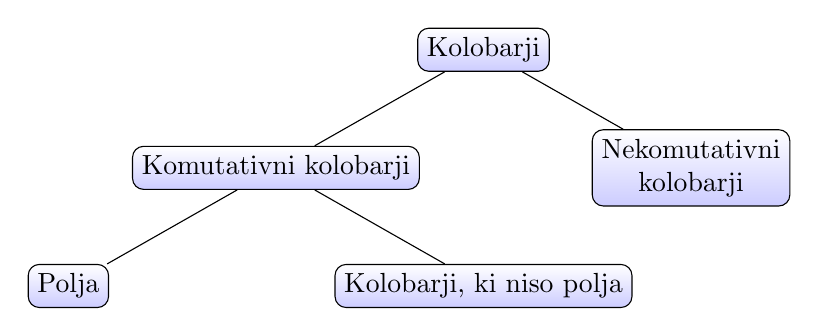
\begin{tikzpicture}[sibling distance=15em,
  every node/.style = {shape=rectangle, rounded corners,
    draw, align=center,
    top color=white, bottom color=blue!20}]]
  \node {Kolobarji}
    child { node {Komutativni kolobarji}
      child { node {Polja} }
      child { node {Kolobarji, ki niso polja} }
    }
    child { node {Nekomutativni \\ kolobarji} };
\end{tikzpicture}
\\
\\
\begin{example}
\begin{example_case}
$\mathbb{Z}$ (tipičen primer kolobarja)
\end{example_case}
\begin{example_case}
$\mathbb{Q}, \mathbb{R}, \mathbb{C}$ (to niso tipični primeri kolobarjev, saj so kar polja)
\end{example_case}
\begin{example_case}
\textbf{Trivialni} ali \textbf{ničelni kolobar}:
$$\{0\}$$
\end{example_case}
\begin{statement}
$$\text{Kolobar} \ \mathcal{K} \ \text{je ničelen} \iff 1=0$$

\begin{proof}\leavevmode \\
$\implies$: Očitno\\
$\impliedby$: $\forall x \in \mathcal{K}. \ x = 1x = 0x = 0$
\end{proof}
\end{statement}
\begin{example_case}
Matrični kolobarji ($M_{n}(\mathbb{R})$, $M_{n}(\mathbb{C})$) z običajnim seštevanjem in množenjem,
$$0 =
	\underbrace{\begin{bmatrix} 
		0 & 0 & \cdots & 0 \\
		0 & \ddots & \ddots & \vdots \\
		\vdots & \ddots & \ddots & 0 \\
		0 & \cdots & 0 & 0		
	\end{bmatrix}}_n; \ 
		1 =	\underbrace{\begin{bmatrix} 
		1 & 0 & \cdots & 0 \\
		0 & \ddots & \ddots & \vdots \\
		\vdots & \ddots & \ddots & 0 \\
		0 & \cdots & 0 & 1
	\end{bmatrix}}_n
$$
Ta kolobar je nekomutativen za $n \geq 2$\\
$ A = \begin{bmatrix}
		1 & 0 \\
		0 & 0
	  \end{bmatrix}
$;
$ B = \begin{bmatrix}
		0 & 1 \\
		0 & 0
	  \end{bmatrix}
$	
$\implies$
$AB = B, \ BA = 0$ \\
$A$ in $B$ ne komutirata, prav tako pa smo videlo da je lahko produkt dveh neničelnih elementov $0$.
\end{example_case}

\begin{definition}
\label{def:left_zero_divisor}
Element $x \neq 0$ kolobarja $\mathcal{K}$, je \textbf{levi delitelj niča}, če obstaja tak $y \neq 0, \in  \mathcal{K}$, da velja: $xy = 0$.
\end{definition}

\begin{definition}
\label{def:right_zero_divisor}
Element $x \neq 0$ kolobarja $\mathcal{K}$, je \textbf{desni delitelj niča}, če obstaja tak $y \neq 0, \in  \mathcal{K}$, da velja: $yx = 0$.
\end{definition}

\begin{definition}
Element $x$ je \textbf{delitelj niča}, če je \textbf{hkrati levi in desni delitelj niča}.
\end{definition}

\begin{remark}
\begin{equation}
\label{eq:left_zero_divisor_iff_right}
\mathcal{K} \ \text{ima leve deljitelje niča} \iff \mathcal{K} \  \text{ima deljitelje niča}
\end{equation}
\begin{proof}\leavevmode \\
$\implies$: Obstajata taka $y \neq 0, x \neq 0$, da je $xy = 0$. Imamo dve možnosti
\begin{enumerate}
\item $yx=0 \implies$ Dokaz je končan.
\item $yx \neq 0$: $x(yx) = 0 = (yx)y$ in je $yx$ desni delitelj niča .
\end{enumerate} 
$\impliedby$: Očitno.
\end{proof}
\end{remark}

V \textbf{Kolobarju brez deliteljev niča} velja:
\begin{equation}
\label{eq:xy_is_zero_implies_one_zero}
\forall x,y \in \mathcal{K}. \ xy = 0 \implies x = 0 \lor y = 0
\end{equation}

V takih kolobarjih velja pravilo krajšanja:
$$ xy = xz \land x  \neq 0 \implies y = z$$
$$ yx = zx \land x  \neq 0 \implies y = z$$
$$ xy = xz \iff x(y-z) = 0$$
$$ yx = zx \iff (y-z)x = 0$$
\end{example}

Kolobar je monoid za množenje zato lahko govorimo o obrnljivih elementih.
\begin{example}
\begin{example_case}
V $\mathbb{Z}$ sta obrnljiva $1, -1$.
\end{example_case}
\begin{example_case}
V $\mathbb{Q}, \mathbb{R}, \mathbb{C}$ so obrnljivi vsi elementi razen $0$
\end{example_case}
\end{example}

\begin{definition}
\label{def:skew_field}
Kolobar, v katerem $1 \neq 0$ in v katerem so \textbf{vsi neničelni elementi obrnljivi} se imenuje \textbf{obseg}.
\end{definition}

\begin{definition}
\label{def:field}
Komutativni obseg se imenuje \textbf{polje}
\end{definition}

\begin{example}
\begin{example_case}
$\mathbb{Q}, \mathbb{R}, \mathbb{C}$, so polja
\end{example_case}
\begin{example_case}
Nekomutativne obsege bomo dodali kasneje
\end{example_case}
\end{example}

\begin{statement}
\label{st:invertible_element_is_not_zero_divisor}
Obrnljiv element kolobarja ni levi(ali desni) delitelj niča.\\
Obsegi so zato kolobarji brez deliteljev niča.
\end{statement}
\begin{proof}
$x$ je obrnljiv: $xy=0$\\
$y = 1y = (x^{-1}x)y =  x^{-1}(xy) = x^{-1}0 = 0$ Torej $x$ ni delitelj niča.
\end{proof}

\subsection{Vektorski prostori}

\begin{definition}
\label{def:vector_space}
Naj bo $\mathcal{F}$ polje. Množica $\mathcal{V}$ skupaj z (notranjo) binarno operacijo seštevanje $+: \mathcal{V} \times \mathcal{V} \to \mathcal{V}$ in zunanjo binarno operacijo $\mathcal{F} \times \mathcal{V} \to \mathcal{V}$ imenovano \textbf{množenje s skalarji} in označeno z $(\lambda, v) \mapsto \lambda v$, se imenuje \textbf{vektorski prostor nad poljem $\mathcal{F}$}, če zanj velja:
\begin{enumerate}[label=\subscript{V}{\arabic*}:]
\item Za seštevanje je $\mathcal{V}$ Abelova grupa
\item Velja distributivnost v vektorskem faktorju
\begin{equation}
\label{eq:vector_space_vector_distributivity}
\forall \lambda \in \mathcal{F}. \  \forall u,v \in \mathcal{V}. \ \lambda(u+v) = \lambda u + \lambda v
\end{equation}
\item Velja distributivnost v skalarnem faktorju
\begin{equation}
\label{eq:vector_space_scalar_distributivity}
\forall \lambda, \mu \in \mathcal{F}. \  \forall v \in \mathcal{V}. \ (\lambda +\mu)v = \lambda v + \mu v
\end{equation}
\item Velja zakon homogenosti
\begin{equation}
\label{eq:vector_space_homogenous}
\forall \lambda, \mu \in \mathcal{F}. \  \forall v \in \mathcal{V}. \ (\lambda \mu)v = \lambda( \mu v)
\end{equation}
\item Enota
\begin{equation}
\label{eq:vector_space_unit}
 \forall v \in \mathcal{V}. \ 1v = v
\end{equation}
\end{enumerate}
\end{definition}

Za vsak vektorski prostor očitno veljajo naslednje trditve

\begin{itemize}
\item $$\forall \lambda \in \mathcal{F}. \ \lambda 0 = 0$$
\item $$\forall u,v \in \mathcal{V}. \  0x = 0$$
\item $$\forall \lambda, \mu \in \mathcal{F}. \  \lambda \mu = 0 \implies \lambda = 0 \lor \mu = 0$$
\item $$\forall \lambda, \mu \in \mathcal{F}. \ (-\lambda) \mu = \lambda(- \mu) = -(\lambda \mu) $$
\end{itemize}

\begin{remark}
Elementom polja $\mathcal{F}$ pravimo \textbf{skalarji}, elementom $\mathcal{V}$ pa vektorji
\end{remark}

\begin{itemize}
\item $\mathcal{F} = \mathbb{R}$: Realni vektorski prostor
\item $\mathcal{F} = \mathbb{C}$: Kompleksni vektorski prostor

\end{itemize}

\begin{example}
\begin{example_case}
Splošni prostor $\mathcal{F}^n$, kjer vpeljemo operaciji:\\
\textbf{Seštevanje}
\begin{equation}
\label{eq:vector_space_addition}
(u_1, u_2, \dots , u_n) + (v_1, v_2, \dots, v_n) \mapsto (u_1 + v_1, u_2 + v_2, \dots, u_n + v_n)
\end{equation}
\textbf{Množenje s skalarjem}
\begin{equation}
\label{eq:vector_space_scalar_multiplication}
\lambda (u_1, u_2, \dots , u_n) \mapsto (\lambda u_1 , \lambda u_2 , \dots, \lambda u_n)
\end{equation}
\end{example_case}
\begin{example_case}
Trivialni vektorski prostor: $\{0\}$
\end{example_case}
\begin{example_case}
Vektorski prostor polinomov stopnje največ $n$, kjer seštevanje in množenje definiramo na običajen način
\end{example_case}
\begin{example_case}
$\mathbb{C}$ je vektorski prostor nad $\mathbb{R}$ ( za $+$ je Abelova grupa, množenje pa definiramo po komponentah, tako je nad $\mathbb{R}$ to $2$-dimenzionalen, nad $\mathbb{C}$ pa $1$-dimenzionalen)
\end{example_case}
\end{example}

\subsection{Algebre}
Mnogi pomembni primeri kolobarjev so hkrati tudi vektorski prostori, dejansko so algebre.

\begin{definition}
\label{def:algebra}
Naj bo $\mathcal{F}$ polje (komutativen obseg). Množica $\mathcal{A}$ skupaj z (notranjima) binarnima operacijama $+$ (seštevanje) in $*$ (množenje) ter zunanjo binarno operacijo $\mathcal{F} \times \mathcal{A} \to \mathcal{A}$ (množenje s skalarji) je \textbf{Algebra na poljem $\mathcal{F}$ ali $\mathcal{F}$-algebra}, če velja:
\begin{enumerate}[label=\subscript{V}{\arabic*}:]
\item Za seštevanje in množenje s skalarji je $\mathcal{A}$ vektorski prostor
\item Za množenje je $\mathcal{A}$ monoid
\item Veljata neke vrste levi in desni distributivnostni zakon
$$\forall x,y,z \in \mathcal{A}. \ \forall \lambda, \mu \in \mathcal{F}. \ (\lambda x + \mu y) z = \lambda(xz) + \mu(yz)$$
$$\forall x,y,z \in \mathcal{A}. \ \forall \lambda, \mu \in \mathcal{F}. \ z(\lambda x + \mu y) = \lambda(zx) + \mu(zy)$$

\begin{remark}
Za $\lambda = \mu = 1$ je to navadna distributivnost. Torej je algebra kolobar, ki je hkrati vektorski prostor, v katerem velja še:
$$\lambda(xz) = (\lambda x)z = x(\lambda z)$$
\end{remark}

\end{enumerate}

\end{definition}


\begin{example}
\begin{example_case}
Vektorski prostor $\mathcal{F}^n$ postane algebra, če definiramo množenje, najlažje kar po komponentah:
\begin{equation}
\label{eq:vector_space_to_algebra_component_mulitplication}
(x_1, x_2, \dots, x_n) (y_1, y_2, \dots, y_n) \mapsto (x_1 y_1,, x_2 y_2, \dots, x_n y_n)
\end{equation} 
\end{example_case}
\begin{example_case}
Kolobar $M_n(\mathbb{R})$ postane algebra, če definiramo množenje s skalarji
\begin{equation}
\label{eq:matrix_scalar_multiplication}
\lambda (a_{ij}) = (\lambda a_{ij})
\end{equation}
\end{example_case}
\begin{example_case}
Vektorski prostor polinomov postane algebra, če vpeljemo množenje polinomov na standardni način
\end{example_case}
\end{example}

\begin{remark}
'Teorija kolobarjev' in 'teorija kolobarjev in algeber' se razlikujeta zgolj v poudarku.
\end{remark}

\subsection{Podgrupe, podkolobarji in druge podstrukture}
$(\mathbb{R}, +)$ in $(\mathbb{C}, +)$ sta različni strukturi, a očitno povezani Abelovi grupi. Operacija je seštevanje in $\mathbb{R} \subseteq \mathbb{C}$. Rečemo: $(\mathbb{R}, +)$ je podgrupa $(\mathbb{C}, +)$. \\
Podobno rečemo 
$(\mathbb{R}, +, *)$ je podkolobar $(\mathbb{C}, +, *)$\\
In ker sta to tudi polji rečemo kar kar $(\mathbb{R}, +, *)$ je podpolje $(\mathbb{C}, +, *)$\\

\subsubsection{Podgrupe}

\begin{definition}
\label{def:subgroup}
\textbf{Neprazna} podmnožica $\mathcal{H}$ grupe $\mathcal{G}$ je \textbf{podgrupa} grupe $\mathcal{G}$, če je za isto operacijo (zožitev na $\mathcal{H} \times \mathcal{H}$) tudi sama grupa. 
\end{definition}

\begin{example}
\begin{example_case}
Vsaka grupa $\mathcal{G}$ ima vsaj dve podgrupi: $\mathcal{G}$ in $\{1\}$\\
\begin{remark}
$\{1\}$ se imenuje \textbf{trivialna podgrupa}
\end{remark}

\begin{remark}
Vsaka od $\mathcal{G}$ različna podgrupa se imenuje \textbf{prava podgrupa}
\end{remark}
\end{example_case}

\end{example}

\begin{statement}
\label{st:subgroup_equivalent_defintions}
Za neprazno podmnožico $\mathcal{H}$ grupe $\mathcal{G}$ so naslednje trditve ekvivalentne:
\begin{enumerate}[label=(\roman*)]
\item $$\mathcal{H} \ \text{je podgrupa} \ \mathcal{G}$$
\item $$\forall x,y \in \mathcal{H}. \ x y^{-1} \in \mathcal{H}$$ 
\item $$\forall x,y \in \mathcal{H}. \ x y \in \mathcal{H} \land x^{-1} \in \mathcal{H}$$ 
\end{enumerate}
\end{statement}
\begin{proof}
\label{pr:subgroup_equivalent_defintions}\leavevmode \\
(i) $\implies$ (ii) : Očitno iz definicije da je $\mathcal{H}$ grupa \\
(ii) $\implies$ (iii) : \\
$$x \in \mathcal{H} \Longrightarrow 1 = x x^{-1} \in \mathcal{H} \Longrightarrow x^{-1} = 1 x^{-1} \in \mathcal{H} \ \text{// Zaprta za inverz}$$
$$x,y \in \mathcal{H} \Longrightarrow x y = x (y^{-1})^{-1} \in \mathcal{H} \ \text{Zaprta za poljubna dva}$$
(iii) $\implies$ (i):\\
Očitno zaprta za množenje, asociativna, ker velja na večji množici ($\mathcal{G}$)
$$1 = x x^{-1} \in \mathcal{H}$$
$$x \in \mathcal{H} \implies x^{-1} \in \mathcal{H}$$
\end{proof}

Govorimo 'grupa $\mathcal{H}$' ali 'podgrupa $\mathcal{H}$' označimo:

$$\mathcal{H} \leq \mathcal{G}$$

\begin{example}
\begin{example_case}
$\mathbb{R} - \{0\}$ je podgrupa $(\mathbb{C}-\{0\})$
\end{example_case}
\begin{example_case}
$\{x \in \mathbb{R} | x < 0\}$ je podgrupa $(\mathbb{C}-\{0\})$
\end{example_case}
\begin{example_case}
$\{1, -1, i, -i\}$ je podgrupa $(\mathbb{C}-\{0\})$
\end{example_case}
\begin{example_case}
$\{z \in \mathbb{C} | \ |z| = 1\}$ je podgrupa $(\mathbb{C}-\{0\})$
\end{example_case}
\begin{example_case}
$\{x \in \mathbb{R} | \ |x| > 1\}$ \textbf{ni} podgrupa $(\mathbb{C}-\{0\})$
\end{example_case}
\begin{example_case}
$\{z \in \mathbb{C} - \{0\} | \ |z| \leq 1\}$ \textbf{ni} podgrupa $(\mathbb{C}-\{0\})$
\end{example_case}
\end{example}

\begin{remark}\\
V aditivni grupi velja \\(ii) :  $\forall x,y \in \mathcal{H}. \ x - y \in \mathcal{H}$ in \\
(iii): $\forall x,y \in \mathcal{H}. \ x + y \in \mathcal{H} \land -x \in \mathcal{H}$
\end{remark}
\\

\begin{example}
Podgrupe $(\mathbb{Z}, +)$\\
\begin{example_case}
Trivialna primera podgrup sta $\mathbb{Z}$ in $\{0\}$
\end{example_case}
\begin{example_case}
$2\mathbb{Z} = \{2n | n \in \mathbb{Z}\}$
\end{example_case}
\begin{example_case}
$k\mathbb{Z} = \{kn | n \in \mathbb{Z}\}$ // $k \in \mathbb{Z}$
\end{example_case}
\end{example}

\begin{definition}
\label{def:conjugate_elements_group}
Elementa $a, b$ iz grupe $\mathcal{G}$ sta si \textbf{konjugirana}, če velja:
\begin{equation}
\label{eq:conjugate_element_group}
\exists c \in \mathcal{G}. \ b = c a c^{-1}
\end{equation}
\begin{remark}
Relacija 'elementa sta si konjugirana' je ekvivalenčna.
\end{remark}
\end{definition}

\begin{statement}
\label{def:conjugate_subgroup}
Če je $c \in \mathcal{H} \leq \mathcal{G}$, je 
\begin{equation}
\label{eq:conjugate_subgroup}
c \mathcal{H} c^{-1} := \{ chc^{-1} | \ h \in \mathcal{H}\}
\end{equation}
\textbf{konjugirana podgrupa} podgrupe $\mathcal{H}$.
\end{statement}

\begin{proof}
\label{st:conjugate_subgroup_is_subgroup}
$$chc^{-1} c h' c^{-1} = c\underbrace{hh'}_{\in \mathcal{H}}c^{-1} \in \mathcal{H}$$
$$(chc^{-1})^{-1}  = (c^{-1})^{-1}h^{-1}c^{-1} = c \underbrace{h^{-1}}_{ \in \mathcal{H}} c^{-1} \in \mathcal{H}$$
\end{proof}

\begin{remark}
Pojem konjugiranih podgrup ima smisel v nekomutativnih grupah
\end{remark}

\subsubsection{Podkolobarji}

\begin{definition}
\label{def:sub_ring}
Podmnožica $\mathcal{L}$ kolobarja $\mathcal{K}$ je \textbf{podkolobar} kolobarja $\mathcal{K}$, če vsebuje enoto \{1\} kolobarja $\mathcal{K}$ in če je kolobar za isti operaciji. 
\end{definition}

\begin{example}
\begin{example_case}
$\mathcal{L} = \{ \begin{bmatrix}
		x & 0 \\
		0 & 0
	  \end{bmatrix} | \ x \in \mathbb{R}\}$\\
	  Sicer je kolobar za isti operaciji, a ne podeduje enote (ima svojo), torej \textbf{ni} podkolobar.
\end{example_case}
\end{example}

\begin{statement}
\label{st:sub_ring_closed_for_inverse}
Podmnožica $\mathcal{L}$ kolobarja $\mathcal{K}$ je podkolobar natanko tedaj, ko velja
\begin{equation}
\label{eq:sub_ring_closed_for_inverse}
1 \in \mathcal{L} \land 
\forall x, y \in \mathcal{L}. \ x-y \in \mathcal{L}
\end{equation}
\end{statement}

\begin{proof}\leavevmode \\
\label{pr:sub_ring_closed_for_inverse}
$\implies$: Sledi iz definicije\\
$\impliedby$ Iz predpostavke sledi, da je $\mathcal{L}$ podgrupa za $+$.\\ Prav tako je $(\mathcal{L}, *)$ monoid\\ Izpolnjevanje distributivnih zakonov pa sledi iz tega da so izpolnjeni tudi na $\mathcal{K}$
\begin{remark}
Uporabili smo trditev (\ref{st:subgroup_equivalent_defintions}) in (ii) pogoj zamenjali z (iii)
\end{remark}
\end{proof}

\begin{example}
\begin{example_case}
Kolobar $\mathbb{Z}$ je podkolobar $\mathbb{Q}$.
\end{example_case}
\begin{example_case}
Kolobar $\mathbb{Q}$ je podkolobar $\mathbb{R}$.
\end{example_case}
\end{example}

\subsubsection{Podprostori}
\begin{definition}
\label{def:vector_subspace}
Podmnožica $\mathcal{U}$ vektorskega prostora $\mathcal{V}$ je \textbf{podprostor} $\mathcal{V}$, če je za isti operaciji tudi sama vektorski prostor.
\end{definition}

\begin{statement}
Za neprazno podmnožico $\mathcal{U}$ vektorskega prostora $\mathcal{V}$ so naslednje trditve ekvivalentne
\begin{enumerate}[label=(\roman*)]
\item $$\mathcal{U} \ \text{je podprostor} \ \mathcal{V}$$
\item $$\forall x, y \in \mathcal{U}. \ \forall \lambda, \mu \in \mathcal{F}. \ \lambda x + \mu y \in \mathcal{U}$$
\item $$\forall x, y, \in \mathcal{U}. \  x + y \in \mathcal{U} \land \forall x \in \mathcal{U}. \  \forall \lambda \in \mathcal{F}. \ \lambda x  \in \mathcal{U}$$
\end{enumerate}	
\end{statement}

\begin{proof}
Očitno
\end{proof}

\begin{example}
Edini podprostori vektorskega prostora $\mathbb{R}^3$ so:
\begin{itemize}
\item $\{0\}$, $\mathbb{R}^3$
\item premice skozi izhodišče
\item ravnine skozi izhodišče
\end{itemize}
\end{example}

\subsubsection{Podalgebre}
\begin{definition}
\label{def:subalgebra}
Podmnožica $\mathcal{B}$ algebre $\mathcal{A}$ je \textbf{podalgebra} $\mathcal{A}$, če je za iste operacije tudi sama algebra in vsebuje enoto \{1\} iz algebre $\mathcal{A}$.
\end{definition}

\begin{statement}
Neprazna podmnožica $\mathcal{B}$ algebre $\mathcal{A}$ je \textbf{podalgebra} algebre $\mathcal{A}$ natanko tedaj ko zanjo velja:
\begin{equation}
\label{eq:is_subalgebra}
1 \in \mathcal{B} \land \forall x, y \in \mathcal{B}. \ \forall \lambda \in \mathcal{F}. \ \underbrace{x+y, \lambda x}_{podprostor}, xy \in \mathcal{B}
\end{equation}
Torej je zaprta za seštevanje, množenje in množenje s skalarji
\end{statement}

\begin{proof}
Enako kot za podkolobarje
\end{proof}

\begin{example}
\begin{example_case}
$A = \mathcal{M}_2(\mathbb{R})$, 
$B = \{ \begin{bmatrix}
		a_{11} & a_{12} \\
		0 	   & a_{22}
	  \end{bmatrix} | a_{ij} \in \mathbb{R} \}$
\leavevmode
\end{example_case}
\end{example}

\subsubsection{Podpolje}

\begin{definition}
\label{def_subfield}
Podmnožica $\mathcal{F}$ polja $\mathcal{E}$ je \textbf{podpolje} polja $\mathcal{E}$, če je za isti operaciji tudi sama polje
\end{definition}

\begin{remark}
Podpolje nujno vsebuje isto enoto $1$ kot polje $\mathcal{E}$, naj bo $e \in \mathcal{F}$ enota.
$e^2 = e \implies e(\underbrace{1}_{enota \ \mathcal{E}}- \ e) = 0$ Ker v poljih ni deliteljev niča, velja $e=1$.
\end{remark}

\begin{statement}
Podmnožica $\mathcal{F} \neq \{0\}$ polja $\mathcal{E}$ je podpolje natanko tedaj ko velja
\begin{equation}
\label{eq:subfield_equivalent_definition}
\forall x, y \in \mathcal{F}. \ xy, x-y \in \mathcal{F} \land 0 \neq x \in \mathcal{F}. \ x^{-1} \in \mathcal{F} 
\end{equation}
\end{statement}

\begin{proof}Podobno kot prej
	
\end{proof}

\begin{statement}
$\mathcal{F} = \{0\} \iff 1 = 0$
\begin{proof}\leavevmode\\
$\implies$

$\forall x \in \mathcal{F}. \ 0x = x$ torej je $0$ nevtralni element

$\impliedby$

$\forall x \in \mathcal{F}. \ x = 1x = 0x = 0$ vsi elementi so ničelni
\end{proof} 
\end{statement}


\begin{definition}
\label{def:field_extension}
Polje $\mathcal{E}$ je \textbf{razširitev} polja $\mathcal{F}$ če je $\mathcal{F}$ podpolje $\mathcal{E}$.
\end{definition}

\begin{example}
\begin{example_case}
$\mathbb{R}$ je podpolje $\mathbb{C}$
\end{example_case}
\begin{example_case}
$\mathbb{C}$ je razširitev $\mathbb{R}$, ki je razširitev $\mathbb{Q}$
\end{example_case}
\end{example}


\subsubsection{Logične operacije nad (pod)strukturami}
Če so $\mathcal{H}_i$ podgrupe grupe $\mathcal{G}$ je tudi njihov presek $\cap \mathcal{H}_i$ podgrupa.

\begin{remark}
Družina $\mathcal{H}_i$ je \textbf{lahko končna ali neskončna} torej poljubna
\end{remark}\\

\textbf{Presek} algebrskih struktur (podgrup, podkolobarjev, podprostorov, podalgeber, podpolji) \textbf{ohrani lastnosti} te algebrske strukture.\\

\textbf{Unija} algebrskih struktur praviloma \textbf{ne ohrani} lastnosti te algebrske strukture.

\begin{example}
\begin{example_case}
$2\mathbb{Z} = \{2n | n \in \mathbb{Z}\}$ in $3\mathbb{Z} = \{3n | n \in \mathbb{Z}\}$ sta podgrupi $\mathbb{Z}$, njuna unija pa ni podgrupa (saj ni grupa), ker $2+3=5 \notin 2\mathbb{Z} \cup 3\mathbb{Z}$
\end{example_case}
\end{example}

\subsection{Generatorji}
$\mathbb{R}^3$ je generiran z vektorji: $(1,0,0), (0,1,0), (0,0,1)$. Edini podprostor, ki te vektorje vsebuje je namreč $\mathbb{R}^3$ sam. Seveda je generiran tudi z drugimi vektorji: $(1,1,0), (0,1,0), (0,0,1)$.\\
Vektorja $(1,0,0),(0,1,0)$ pa generirata ravnino: $z=0$.

\subsubsection{Generatorji grup}
Naj bo $\mathcal{X}$ neprazna podmnožica grupe $\mathcal{G}$, Vzemimo množico vseh elementov oblike $x_1 x_2 \dots x_n$, kjer velja $x, x^{-1} \in \mathcal{X}$ in jo označimo z $<\mathcal{X}>$.
 
Če je $\mathcal{X} = \{y_1, y_2, \dots , y_n\}$ pišemo tudi $\mathcal{X} = <y_1, y_2, \dots , y_n>$. 

Tako $<x,y>$ sestoji iz elementov kot so: $1, x, y, x^2, x^3, x^{-1}, x^{-2}, x^{-1}y, y^{-1}, x^5y^{-1}x^3y^{-3}xy^2, \dots$
\textbf{Opazimo}, da je $<\mathcal{X}>$ podgrupa
$$u,v \in <x> \implies uv \in <\mathcal{X}> \land u^{-1} \in <x>$$
$(x_1,\dots, x_n)^{-1} = x_{1}^{-1} \dots x_n^{-1}$, ki vsebuje množico $\mathcal{X}$.

Velja pa tudi obratno: vsaka podgrupa grupe $\mathcal{G}$, ki vsebuje $\mathcal{X}$ vsebuje tudi to podgrupo($<\mathcal{X}>$).

Torej je $<\mathcal{X}>$ najmanjša podgrupa, ki vsebuje $\mathcal{X}$. Pravimo ji \textbf{podgrupa, generirana z $\mathcal{X}$}.

Če velja $<\mathcal{X}> = \mathcal{G}$, rečemo, da je $\mathcal{G}$ generirana z množico $\mathcal{X}$, elemente iz $\mathcal{X}$ pa imenujemo \textbf{generatorji} grupe $\mathcal{G}$, množici $\mathcal{X}$ pa \textbf{množica generatorjev}.\\

\begin{example}
\begin{example_case}
$\mathbb{Q}^+$ je grupa za množenje. Velja: $<\mathbb{N}> = \mathbb{Q}^+$
\end{example_case}
\begin{example_case}
$<2,3> = \{2^i 3^j | i,j \in \mathbb{Z}\}$
\end{example_case}
\end{example}

\begin{remark}
V aditivni grupi $<\mathcal{X}>$ za komponiranje elementov uporabljamo drugo operacijo, vse ostalo ostane isto.
\end{remark}\\

\begin{example}
\begin{example_case}
Grupa $(\mathbb{Z}, +)$ je generirana z $<1>$ in prav tako tudi z $<-1>$. Velja $\mathbb{Z} = <1> = <-1>$.
\end{example_case}
\end{example}

\begin{remark}
Grupe generirane z enim samim elementom imenujemo \textbf{ciklične}.($<2> = <4,6> = 2\mathbb{Z}$)

\end{remark}

Cilj je poiskati najmanjše množice generatorjev(očitno $<\mathcal{G}> = \mathcal{G}$).

\begin{definition}
\label{def:finitly_generated_group}
Grupa je \textbf{končno generirana} če je generirana s kako končno množico.
\end{definition}

\subsubsection{Generatorji kolobarja}
Naj bo $\mathcal{K}$ kolobar, $\emptyset \neq \mathcal{X} \subseteq \mathcal{K}$.

Označimo z $\overline{\mathcal{X}}$ podgrupo za seštevanje $\mathcal{K}$, ki vsebuje vse produkte elementov iz $\mathcal{X} \cup \{1\}$.

Opazimo: $\overline{\mathcal{X}}$ je podkolobar, ki vsebuje $\mathcal{X}$ in je vsebovan v vsakem podkolobarju, ki $\mathcal{X}$ vsebuje. Zato mu rečemo \textbf{podkolobar generiran z množico $\mathcal{X}$}.

\begin{example}
\begin{example_case}
$\mathcal{K} = \mathbb{C}$
\begin{itemize}
\item $\overline{\{1\}} = \mathbb{Z}$
\item $\overline{\{i\}} = \{ n + mi | n,m \in \mathbb{Z}\} = \mathbb{Z}[i]$ (Kolobar \textbf{Gaussovih celih števil})
\end{itemize}\leavevmode
\end{example_case}
\end{example}

\begin{remark}
Pojme, kot so \textbf{generator kolobarja, končno generiran kolobar,\dots} definiramo enako kot za grupo.
\end{remark}

\subsubsection{Generatorji vektorskih prostorov}

\begin{definition}
\label{def:linear_combination}
Naj bo $\mathcal{V}$ vektorski prostor nad $\mathcal{F}$. Vsakemu vektorju $v$ oblike
\begin{equation}
\label{eq:linear_combination}
v = \lambda_1 v_1 + \dots + \lambda_n v_n; \lambda_i \in \mathcal{F} \land v_i \in \mathcal{V}
\end{equation}
pravimo \textbf{linearna kombinacija} vektorjev $v_1, v_2, \dots, v_n$.
\end{definition}


\begin{definition}
\label{def:linear_spang_enerated}Naj bo 
$\emptyset \neq \mathcal{X} \subseteq \mathcal{V}$. Podprostor generiran z $\mathcal{X}$, torej podprostor, ki $\mathcal{X}$ vsebuje in je vsebovan v vsakem podprostoru, ki vsebuje $\mathcal{X}$, je množica $\mathcal{L}(\mathcal{X})$, vseh linearnih kombinacij vektorjev iz $\mathcal{X}$, $\mathcal{L}(\mathcal{X})$ imenujemo \textbf{linearna lupina množice $\mathcal{X}$}.
\end{definition}


\begin{definition}
Naj bo $\mathcal{X}$ množica generatorjev za $\mathcal{V}$, tedaj $\mathcal{X}$ imenujemo \textbf{ogrodje $\mathcal{V}$}. Velja še $\mathcal{L}(\mathcal{X}) = \mathcal{V}$.
\end{definition}

\begin{remark}
Posebnost vektorskega prostora je v tem, da imamo pojem \textbf{linearne neodvisnosti}, preko katerega vpeljemo pojem \textbf{baze} vektorskega prostora.
\end{remark}


\subsubsection{Generatorji algeber}

\begin{definition}
\label{def:subalgebra_generated}
Naj bo $\mathcal{A}$ algebra na $\mathcal{F}$, naj bo $\emptyset \neq \mathcal{X} \subseteq \mathcal{A}$. \textbf{Podalgebra generirana z $\mathcal{X}$} je množica, ki sestoji iz elementov $x$ oblike
\begin{equation}
\label{eq:subalgebra_generated_element}
x = \lambda_1 x_{11} x_{12} \dots x_{1n_1} + \dots + \lambda_r x_{r1} x_{rn_r}; \lambda_i \in \mathcal{F} \land x_i \in \mathcal{X} \cup \{1\}
\end{equation}
\end{definition}



\begin{example}
\begin{example_case}
$\mathcal{A} = \mathcal{M}_2(\mathbb{R})$ 
\begin{itemize}
\item Podalgebra generirana z:

$e_{11} = \begin{bmatrix}
		1 & 0 \\
		0 & 0
	  \end{bmatrix}$, 
$e_{22} = \begin{bmatrix}
		0 & 0 \\
		0 & 1
	  \end{bmatrix}$
	  
je algebra diagonalnih matrik: 
$$\begin{bmatrix}
	   \lambda & 0 \\
		0 & \mu
		
	  \end{bmatrix}; \ \lambda, \mu \in \mathbb{R}$$ 
\item Podalgebra generirana z:

$e_{11} = \begin{bmatrix}
		0 & 1 \\
		0 & 0
	  \end{bmatrix}$, 
$e_{22} = \begin{bmatrix}
		0 & 0 \\
		1 & 0
	  \end{bmatrix}$
	  
pa je celotna algebra $\mathcal{M}_2(\mathbb{R})$ (torej je generirana samo z dvema elementoma).

Ker velja:

$e_{12} e_{21} = e_{11}$ in $e_{21} e_{12} = e_{22}$, vidimo, da $e_{12}, e_{21}$ generirata algebro $\mathcal{M}_2(\mathbb{R})$.  
$\{e_{12}, e_{21}, e_{11}, e_{22} \}$ je baza algebre $\mathcal{M}_2(\mathbb{R})$

\begin{remark}

Za primerjavo: podkolobar $\mathcal{M}_2(\mathbb{R})$ generiran z $e_{12}$ in $e_{21}$ pa je 

$\mathcal{M}_2(\mathbb{Z})= \begin{bmatrix}
		u_{11} & u_{12} \\
		u_{21} & u_{22}
	  \end{bmatrix}; u_{ij} \in \mathbb{Z}$
\end{remark}
\end{itemize}\leavevmode
\end{example_case}
\end{example}

\subsubsection{Generatorji podpolj}
\begin{definition}
\label{def:subfield_generated}
Naj bo $\mathcal{X} \neq \emptyset$ podmnožica polja $\mathcal{F}$. \textbf{Podpolje generirano z $\mathcal{X}$} je množica
\begin{equation}
\label{eq:subfield_genrated_element}
\{uv^{-1} | u,v \in \overline{\mathcal{X}} \land v \neq 0\}
\end{equation}
\end{definition}

\begin{remark}
Podkolobar $\overline{\mathcal{X}}$ generiran z $\mathcal{X}$ ni nujno polje.
\end{remark}

Očitno vsako podpolje, ki $\mathcal{X}$ vsebuje, vsebuje tudi podpolje generirano z $\mathcal{X}$, toda zakaj ta množica je podpolje?.

Pomembno je dokazati, da je podgrupa za seštevaje (zaprtost za množenje, inverz, in 1 so očitne)
\begin{statement}
\label{st:generated_subfield_is_subgroup}
$$uv^{-1} - wz^{-1} = \underbrace{(uz - vw)}_{\in \overline{\mathcal{X}}} \underbrace{(vz)^{-1}}_{\in \overline{\mathcal{X}}}$$
\end{statement} 

\begin{example}
$\mathcal{F} = \mathbb{C}$

\begin{example_case}
$\mathcal{X} = \{1\}$ Podpolje generirano z $\mathcal{X}$ je $\mathbb{Q}$, medtem, ko $\overline{\mathcal{X}} = \mathbb{Z}$
Vsako podpolje $\mathbb{C}$ vsebuje $1$ in zato vsako podpolje vsebuje tudi $\mathbb{Q}$
\end{example_case}
\begin{example_case}
$\mathcal{X} = {i}$:  $\overline{\mathcal{X}} = \mathbb{Z}[i]$(Gaussova cela števila), podpolje generirano z $\mathcal{X}$ je 
\begin{equation}
\label{eq:rational_imag_generated}
\mathbb{Q}[i] := \{p + qi | p,q \in \mathbb{Q}\}
\end{equation}
\end{example_case}
\end{example}

\begin{remark}
Med drugim smo pokazali, da najmanjša podgrupa (podkolobar $\dots$), ki vsebuje dano množico, res obstaja. Zadevo pa lahko dokažemo tudi hitreje, tako da vzamemo presek vseh podstruktur, ki to strukturo vsebujejo.
\end{remark}

\subsection{Direktni produkti in vsote}
Iz danih struktur lahko konstruiramo nove na različne načine.
\subsubsection{Direktni produkti grup}

\begin{definition}
\label{def:outer_direct_product_of_groups}
Naj bodo $\mathcal{G}_1, \dots, \mathcal{G}_n$ grupe. Grupi $$\mathcal{G} := \mathcal{G}_1 \times \dots \times \mathcal{G}_n$$ ki jo dobimo kot kartezični produkt teh grup, pravimo \textbf{(zunanji) direktni produkt}.
\end{definition}

\begin{remark}
Da je ta struktura res grupa, operacijo definiramo po komponentah. Brez težav se prepričamo, da je to res grupa.
$$(x_1, x_2, \dots, x_n) * (y_1, y_2, \dots, y_n) := (x_1 y_1, x_2 y_2, \dots, x_n y_n)$$
Očitno:
$$1 = (1,1, \dots, 1)$$
$$(x_1, x_2, \dots, x_n)^{-1} = (x_1^{-1}, x_2^{-1}, \dots, x_n^{-1})$$
\end{remark}

\begin{remark}
Če so vse grupe v produktu aditivne, potem namesto $\mathcal{G} := \mathcal{G}_1 \times \dots \times \mathcal{G}_n$ pišemo $\mathcal{G} := \mathcal{G}_1 \oplus \dots \oplus \mathcal{G}_n$ in govorimo o \textbf{(zunanji) direktni vsoti grup}.
\end{remark}

\subsubsection{Direktni produkti kolobarjev}

\begin{definition}
\label{def:outer_direct_product_of_rings}
Naj bodo $\mathcal{K}_1, \dots, \mathcal{K}_n$ kolobarji. Kolobarju $$\mathcal{K} := \mathcal{K}_1 \times \dots \times \mathcal{K}_n$$ ki ga dobimo kot kartezični produkt teh kolobarjev, pravimo \textbf{(zunanji) direktni produkt}.
\end{definition}

\begin{remark}
Da je ta struktura res kolobar, operacijo definiramo po komponentah. Brez težav se prepričamo, da je to res kolobar.
$$(x_1, x_2, \dots, x_n) + (y_1, y_2, \dots, y_n) := (x_1 + y_1, x_2 + y_2, \dots, x_n + y_n)$$
$$(x_1, x_2, \dots, x_n) * (y_1, y_2, \dots, y_n) := (x_1 y_1, x_2 y_2, \dots, x_n y_n)$$
\end{remark}

\begin{remark}
Temu rečemo tudi \textbf{direktna (zunanja) vsota kolobarjev}.
\end{remark}

\subsubsection{Direktna vsota vektorskih prostorov}

\begin{definition}
\label{def:direct_sum_of_vector_spaces}
Naj bodo $\mathcal{V}_1, \dots, \mathcal{V}_n$ vektorski prostori nad $\mathcal{F}$. Vektorskemu prostoru $$\mathcal{V} := \mathcal{V}_1 \times \dots \times \mathcal{V}_n$$ ki ga dobimo kot kartezični produkt teh vektorskih prostorov, pravimo \textbf{direktna vsota} prostorov $\mathcal{V}_1, \dots, \mathcal{V}_n$ in ga označujemo kot $\mathcal{V}_1 \oplus \dots \oplus \mathcal{V}_n$.
\end{definition}

\begin{remark}
Da je ta struktura res vektorski prostor, operacijo definiramo po komponentah. Brez težav se prepričamo, da je to res vektorski prostor.
$$(x_1, x_2, \dots, x_n) + (y_1, y_2, \dots, y_n) := (x_1 + y_1, x_2 + y_2, \dots, x_n + y_n)$$
$$\lambda(x_1, x_2, \dots, x_n) := (\lambda x_1, \lambda x_2, \dots, \lambda x_n)$$
\end{remark}

\begin{remark}
$\mathcal{F}^{n}$ je direktna vsota $n$-kopij enorazsežnega prostora $\mathcal{F}$
\end{remark}



\subsubsection{Direktni produkt algebr}

\begin{definition}
\label{def:direct_product_of_vector_algebras}
Naj bodo $\mathcal{A}_1, \dots, \mathcal{A}_n$ algebre nad $\mathcal{F}$. Algebri $$\mathcal{A} := \mathcal{A}_1 \times \dots \times \mathcal{A}_n$$ ki jo dobimo kot kartezični produkt teh algebr, pravimo \textbf{direktni produkt}.
\end{definition}

\begin{remark}
Da je ta struktura res algebra, operacijo definiramo po komponentah. Brez težav se prepričamo, da je to res algebra.
$$(x_1, x_2, \dots, x_n) + (y_1, y_2, \dots, y_n) := (x_1 + y_1, x_2 + y_2, \dots, x_n + y_n)$$
$$(x_1, x_2, \dots, x_n) * (y_1, y_2, \dots, y_n) := (x_1 y_1, x_2 y_2, \dots, x_n y_n)$$
$$\lambda(x_1, x_2, \dots, x_n) := (\lambda x_1, \lambda x_2, \dots, \lambda x_n)$$
\end{remark}

\begin{remark}
Lahko govorimo tudi o direktnem produktu(direktni vsoti) neskončne družine struktur
\end{remark}

\begin{example}
\begin{example_case}
$\mathbb{R}$ glejmo kot algebro nad $\mathbb{R}$. Direktni produkt števno kopij z operacijami po komponentah je algebra $\mathbb{R} \times \mathbb{R} \times \dots$.

Operacije po komponentah točno sovpadajo z operacijami po komponentah za zaporedja. To je torej algebra realnih zaporedij.
\end{example_case}
\begin{example_case}
Naj bodo $\mathcal{F}_1, \dots, \mathcal{F}_n$ polja nad ne nujno istimi kolobarji. Definiramo operacije po komponentah in opazimo, da za $n \geq 2$ ima direktni produkt(polj ali kolobarjev) delitelje niča.
$$(x_1, 0, \dots , 0) * (0, x_2, x_3, \dots, x_n) = 0$$
\end{example_case}

\end{example}

\section{Primeri grup in kolobarjev}
\subsection{Cela števila}
Ker so $\mathbb{N}$ zgolj polgrupa za $+$, imamo v algebri raje $\mathbb{Z}$.

\begin{definition}
\label{def:total_ordering}
Množica $\mathcal{A}$ zadostuje \textbf{načelu dobre urejenosti}, če vsaka neprazna navzdol omejena podmnožica množice $\mathcal{A}$, vsebuje najmanjši element.
\end{definition}

\begin{remark}
Je ekvivalentno:

Če v množici $\mathcal{A}$, ki ustreza načelu dobre urejenosti, množica $\mathcal{B} \subseteq \mathcal{A}$ nima najmanjšega elementa, potem velja $\mathcal{B} = \emptyset$
\end{remark}

\begin{statement}
$\mathbb{N}$ ustreza načelu dobre urejenosti.
\end{statement}
\begin{proof}\leavevmode\\
Z indukcijo na $n$:
$n=1$: $1 \notin \mathbb{N}$

$n \implies n+1$: $1 \notin \mathbb{N}, 2 \notin \mathbb{N}, \dots, n \notin \mathbb{N} \underbrace{\implies}_{\text{Ker nima najmanjšega elementa}} n+1 \notin \mathbb{N}$
\end{proof}

Po indukciji isto velja tudi za $\mathbb{N} \cup \{0\}$, $\mathbb{N} \cup \{0, -1\}$, $\mathbb{N} \cup \{0, -1, -2\}$ $\dots$


Torej: Vsaka neprazna navzdol omejena podmnožica $\mathbb{Z}$ vsebuje najmanjše število.

Analogno: Vsaka neprazna navzgor omejena podmnožica $\mathbb{Z}$ vsebuje največje število.
\\

\begin{theorem}[Osnovni izrek o deljenju]
Za poljubna $m,n \in \mathbb{Z}$ obstajata taki števili $p,q \in \mathbb{Z}$, da velja:
$$m = qn + r \land 0 \leq r < n$$
\end{theorem}

\begin{proof}
Vpeljimo
$$\mathcal{S}_{(n,m)} := \{k \in \mathbb{Z} | kn \leq m\}$$
Če $\mathcal{S} = \emptyset $ $\checkmark$ 
$\mathcal{S}$ je navzgor omejena, ker lahko najdemo tako število $k$, tako da je $kn > m$ in to velja tudi za vsako od $k$ večje število, zato $\mathcal{S}$ vsebuje največje število $q$. Tako velja
$$qn \leq m \ \ // \ \text{saj} \ q \in \mathcal{S}$$
$$(q + 1)n > m \ \ // \ \text{saj} \ (q + 1) \notin \mathcal{S}$$
$$r:= m-qn \geq 0$$
$$qn + n > m \ \ // \ \text{torej} \ n > r$$
\end{proof}

\begin{remark}
$r$ imenujemo \textbf{ostanek} pri deljenju $m$ z $n$.
\end{remark}
\\

$(\mathbb{Z}, +)$
Primeri podgrup

\begin{example}
\begin{example_case}
Trivialni primeri: $\{0\}$, $\mathbb{Z}$
\end{example_case}
\begin{example_case}
$n\mathbb{Z} = \{nk | k \in \mathbb{Z}\}$ // $n \in \mathbb{Z}$ je podgrupa za seštevanje

\begin{remark}
Ker $n\mathbb{Z} = (-n)\mathbb{Z}$, praviloma izberemo $n \in \mathbb{N}$
\end{remark}
\end{example_case}
\end{example}

\begin{theorem}
\label{th:only_aditive_subgroup_of_integers}Podmnožica $\mathcal{H}$ množice $\mathbb{Z}$ je podgrupa za seštevanje natanko tedaj, ko obstaja tak $n \geq 0$, da je $\mathcal{H} = n\mathbb{Z}$.
\end{theorem}

\begin{proof}\leavevmode\\
$\implies$\\
$\mathcal{H}$ je podgrupa $\mathbb{Z}$\\ $\mathcal{H} = \{0\} \implies n = 0$\\
$\mathcal{H} \neq \{0\}$, $k \in \mathcal{H} \iff -k \in \mathcal{H} \implies \mathcal{H} \cap \mathbb{N} \neq \emptyset$
Po načelu dobre urejenosti obstaja najmanjše število v $\mathcal{H}$, recimo mu $n$.\\
$n \in \mathcal{H} \implies n\mathbb{Z} \subseteq \mathcal{H} \ //\text{ker je podgrupa}$\\
Vzemimo sedaj: $m \in \mathcal{H} \implies \underbrace{r}_{\in \mathcal{H}} = \underbrace{m}_{\in \mathcal{H}} - \underbrace{qn}_{\in \mathcal{H}}$\\
In dobimo $r = 0$, ker iz $1 \leq r \leq n-1$ sledi, da $\mathcal{H}$ vsebuje od $n$ manjše število, kar je protislovje.\\
Torej
$m = qn \in \mathcal{H}$\\
$\impliedby$\\
$n\mathbb{Z}$ je podgrupa $\implies (nk - nl) = n(k-l) \in n\mathbb{Z}$

\end{proof}

\begin{definition}
\label{def:divisor_integers}
Naj bosta $m,k \in \mathbb{Z}$. Rečemo, da \textbf{$k$ deli $m$} (pišemo tudi $k|m$), če obstaja tak $q \in \mathbb{Z}$, da velja $m = qk$.
\end{definition}

\begin{remark}
Rečemo tudi $m$ \textbf{je deljiv} s $k$ ali $k$ je \textbf{delitelj} $m$. Prav tako uporabljamo $k \nmid m$, da povemo, da $k$ \textbf{ne deli} $m$.
\end{remark}


\begin{definition}
\label{def:gcd_integers}
Naj bosta $m,n \in \mathbb{Z}$, naravno število $d$ je \textbf{največji skupni delitelj} $m$ in $n$, če velja:
\begin{enumerate}
\item $d|m \land d|n$
\item $\forall d' \in \mathbb{N}. \ d'|m \land d'|n \implies d'|d \ //$ Vsak drugi skupni delitelj deli največji skupni delitelj
\end{enumerate} 
\end{definition}


\begin{remark}
Če sta $\mathcal{H}$ in $\mathcal{K}$ podgrupi aditivne grupe $\mathcal{G}$, je podgrupa tudi
$$\mathcal{H} + \mathcal{K} := \{h+k | h \in \mathcal{H}, k \in \mathcal{K}\}$$
Očitno $\mathcal{H}, \mathcal{K} \subseteq \mathcal{H} + \mathcal{K}$, to je tudi najmanjša podgrupa, ki vsebuje obe podgrupi.
\end{remark}

\begin{proof}
$$(h+k) - (h' + k') = (h - h') + (k - k') \in \mathcal{H} + \mathcal{K}$$
\end{proof}

\begin{theorem}
\label{th:existance_of_gcd}Za vsak par celih števil $m,n$, od katerih vsaj eno ni enako $0$, obstaja največji skupni delitelj $d$, ki ga označimo z $gcd(m,n)$, in je oblike $d= mx + ny$ za neka $x,y \in \mathbb{Z}$.
\end{theorem}

\begin{proof}
$m\mathbb{Z}$ in $n\mathbb{Z}$ sta podgrupi $\mathbb{Z}$, zato je tudi njuna vsota podgrupa. Po opombi zgoraj obstaja tak $d \in \mathbb{N}$, da velja $d\mathbb{Z} = m\mathbb{Z} + n\mathbb{Z}$ in ker eno izmed $m,n$ ni $0$ velja $d \neq 0$. Torej velja\\
$d = mx + ny$ za neka $x,y \in \mathbb{Z}$ Torej velja:\\ $d \mathbb{Z} \supseteq m\mathbb{Z} \implies m \in m\mathbb{Z} \subseteq d\mathbb{Z} \implies d|m$ in podobno za $n$.
Dokazali smo, da je $d$ skupni delitelj števil $m$ in $n$. Potrebno je še dokazati, da je največji.\\
Naj velja $c|m$ in $c|n$, potem $m=cz$ in $n=cw$.\\
Vemo da $d = mx + ny = c(zx + wy) \implies c|d$
\end{proof}

\begin{remark}
Dokaz za to se pojavi že v Evklidovi knjigi Elementi, približno 300 let pr. Kr.
\end{remark}

\begin{definition}
\label{def:coprime_integers}
Števili $m,n \in \mathbb{Z}$, ne obe enaki $0$, sta si \textbf{tuji}, če je njun največji skupni delitelj enak $1$. 
\end{definition}


\begin{corollary}
Celi števili $m,n$ sta si tuji natanko tedaj, ko obstajata taki celi števili $x,y$, ki zadostita enačbi:
$$1=mx + ny$$
\end{corollary}

\begin{proof}\leavevmode\\
$\implies$ \\Sledi iz izreka o obstoju največjega skupnega delitelja (\ref{th:existance_of_gcd})\\
$\impliedby$\\
$c|m \land c|n \implies c|1$ Torej je njun največji skupni delitelj 1 in sta si tuji. 
\end{proof}

\begin{remark}
Splošneje lahko definiramo največji skupni delitelj števil $n_1, n_2, \dots, n_k \in \mathbb{Z}$ na enak način ter njegovo eksistenco dokažemo na enak način ($d=n_1x_1 + n_2x_2 + \dots n_kx_k$). To seveda ne pomeni, da so si števila paroma tuja ($2,3,6$ so si tuja, ne pa tudi paroma tuja).
\end{remark}

\begin{definition}
\label{def:prime}
Naravno število $p$ je \textbf{praštevilo}, če sta $1$ in $p$ edini naravni števili, ki ga delita in velja $p \neq 1$.
\end{definition}

\begin{lemma}
\label{lem:prime_divisibility}
Naj bo $p$ praštevilo in $mn \in \mathbb{Z}$, tedaj velja:
$$p |mn \implies p|m \lor p|n$$
\end{lemma}

\begin{proof}
Predpostavimo, da $p\nmid m$.\\
$gcd(p,m) = 1 \implies 1 = px + my \implies n = pxn + \underbrace{mn}_{pz}y = p(xn + zy)$ \\
Podobno za drugo možnost.
\end{proof}

\begin{remark}
Tudi ta dokaz je bil poznan že Evklidu.
\end{remark}

\begin{theorem}[Osnovni izrek aritmetike]
\label{th:fundamental_theroem_of_arithmetics}Vsako naravno število $n \geq 2$ lahko zapišemo kot produkt praštevil. Ta zapis je do vrstnega reda faktorjev natančno enoličen.
\end{theorem}

\begin{proof}
Indukcija na $n$:\\
$n = 2 \ \checkmark$\\
$n-1 \implies n$\\
Če je $n$ praštevilo je dokaz zaključen. Če ni, ima vsaj dva delitelja ki nista $1$ ali $p$ (lahko sta enaka).\\
$n = kl;\  l,k < n$ \\
Po indukcijski predpostavki sta $l$ in $k$ produkta praštevil, torej je tudi $p$ produkt praštevil.\\
In še edinost zapisa:\\
$n = p_1 * p_2 * \dots * p_r = q_1 * q_2 * \dots * q_s$, produkt samih praštevil\\
$p_1 | q_1 * q_2 * \dots * q_s$ torej po lemi (\ref{lem:prime_divisibility}) deli natančno enega izmed faktorjev $q_i$. Brez škode za splošnost: $p_1|q_1 \underbrace{\implies}_{\text{ker sta praštevili}} p_1 = q_1$ Krajšamo s $p_1$ in nadaljujemo dokler ne pridemo do $1=1$.\\
Če pa imamo $s > r \implies q_{r+1}\dots q_s = 1$, kar pa je protislovje.
\end{proof}

\begin{theorem}
\label{th:infinite_number_of_primes}
Množica praštevil je neskončna.
\end{theorem}

\begin{proof}
Predpostavimo, da jih je končno, torej da so $p_1, p_2, \dots, p_n$ vsa praštevila. Tedaj $p_1*p_2*\dots * p_n + 1$ ni praštevilo in je zato gotovo deljivo z nekim praštevilom $p_i$.\\
$p_1*p_2*\dots * p_n + 1 = k*p_i \implies p_i(k - p_1*p_2*\dots *p_{i-1} * p_{i+1} * \dots * p_n) = 1$, protislovje.
\end{proof}

\subsection{Grupa in kolobar ostankov}

\begin{definition}
\label{def:modulo_congruent}
Celi števili $a$ in $b$ sta \textbf{kongruenti modulo $n$}, če $$n|(a-b)$$
\end{definition}

\begin{example}
\begin{example_case}
$13 \equiv  1 \ (\textrm{mod}\ 12)$, $21 \equiv -3 \ (\textrm{mod}\ 12)$
\end{example_case}
\begin{example_case}
$a \equiv b \ (\textrm{mod}\ 1)$
\end{example_case}
\end{example}

\begin{lemma}
\label{lem:modulo_equivalence_addition}
$$a \equiv a' \ (\textrm{mod}\ n) \land b \equiv b' \ (\textrm{mod}\ n) \implies a+b \equiv a'+b' \ (\textrm{mod}\ n) \land ab \equiv a'b' \ (\textrm{mod}\ n)$$
\end{lemma}

\begin{proof}
$$(a+b) - (a' + b') = \underbrace{(a-a') + (b-b')}_{\text{sta si kongruentna}}$$
$$(ab) - (a' b') = \underbrace{b(a-a') + a'(b-b')}_{\text{sta si kongruentna}}$$
\end{proof}

\begin{statement}
Relacija $a \equiv b \ (\textrm{mod}\ n)$ je ekvivalenčna:
\end{statement}

\begin{proof}\leavevmode\\
Refleksivna: $\checkmark$\\
Simetrična: $\checkmark$\\
Tranzitivna:\\
$a \equiv b \ (\textrm{mod}\ n)$ in $b \equiv c \ (\textrm{mod}\ n)$ $\implies c-a = \underbrace{(c-b) + (b-a)}_{\text{sta si kongruentna}}$
\end{proof}

Ker je relacija ekvivalenčna, lahko vpeljemo ekvivalenčne razrede. Z $[a]$ označimo ekvivalenčni razred, ki mu pripada $a$.

\begin{definition}
\label{def:equivalence_classes_modulo}
Ekvivalenčni razredi kongurgento z $n$ so:
$$\underbrace{[0]}_{\text{števila deljiva z }n} , \underbrace{[1]}_{\text{ostanek pri deljenji z }n \ \text{je }1}, \dots , [n-1]$$
in jih označimo z $\mathbb{Z}_n$.
%Se da tole kaj lepše zapisat, malce razpotegnjeno je vse, pa spodaj je dosti skupaj komentar.
\end{definition}

Potrebno je preveriti še dobro definiranost operacij.
\\
\\
\begin{statement}
Če v množici $\mathbb{Z}_n$ vpeljemo seštevanje:
\begin{equation}
\label{eq:def_modulo_adition}
[a] + [b] := [a+b]
\end{equation}
Postane $\mathbb{Z}_n$ Abelova grupa.
\end{statement}

\begin{proof}
Dobra definiranost seštevanja:\\
$$ \underbrace{[a] = [a']}_{a \equiv a' \ (\textrm{mod}\ n)} \land \underbrace{[b] = [b']}_{b \equiv b' \ (\textrm{mod}\ n)} \implies [a+b] = [a' + b']$$ 
Drugi del izjave pa je ekvivalenten: $a+b \equiv a' + b'\ (\textrm{mod}\ n)$, kar sledi iz leme (\ref{lem:modulo_equivalence_addition}).
\\\\
Preverimo še asociativnost:
$$([a] + [b]) + [c] = [a + b] + [c] \underbrace{=}_{\text{po definiciji}} \underbrace{[(a+b) + c] = [a + (b + c)] =}_{\text{asociativnost celih števil}} \dots = [a] + ([b] + [c])$$
Nevtralni element:
$$0 = [0]$$
Nasprotni element:
$$-[a] = [-a]$$
Komutativnost:
$$[a] + [b] = [a+b] = [b+a] = [b] + [a]$$
\end{proof}


\begin{statement}
Aditivna grupa $\mathbb{Z}_n$ postane\textbf{komutativen kolobar} $\mathbb{Z}_n$, če vpeljemo množenje s predpisom:
\begin{equation}
\label{eq:def_modulo_group_multiplication}
[a]*[b] := [a*b]
\end{equation}
\end{statement}

\begin{proof}\leavevmode\\
Dobra definiranost sledi iz leme(\ref{lem:modulo_equivalence_addition}), asociativnost in distributivnost pokažemo kot pri seštevanju (se sklicujemo na te lastnosti v celih številih).\\
Enota: $[1]$
\end{proof}


\begin{remark}
Da oznake poenostavimo, namesto $[a], 0 \leq a \leq n-1$ pišemo kar $a$, in tako $\mathbb{Z}_n = \{0,1, \dots, n-1\}$, pri čemer moramo obdržati v mislih, da to niso 'prava' cela števila.
\end{remark}

Vsoto $a+b$ izračunamo tako, da pogledamo ostanek pri deljenju običajne vsote, podobno s produktom.

\begin{example}
\begin{example_case}
V $\mathbb{Z}_{12}$: $3+4 = 7$ in $3+11 = 2 + 1*12 = 2$ ter $3*7 = 9$ in $3*8 = 0$.\\
$\mathbb{Z}_n$ ima torej lahko delitelje niča. Očitno je to res vedno, kadar je $n$ sestavljeno število. Če pa je $n$ praštevilo, pa to ni res, še več, $\mathbb{Z}_p$ je polje.
\end{example_case}
\end{example}

\begin{definition}
\label{def:full_ring}
Komutativen kolobar brez deliteljev niča se imenuje \textbf{cel kolobar}.
\end{definition}

\begin{example}
$\underbrace{\mathbb{Z}}_{\text{cel kolobar, ki ni polje}}, \mathbb{Q}, \mathbb{R}, \mathbb{C}$
\end{example}


\begin{statement}
\label{st:finite_full_ring_is_field}
Končen cel kolobar je polje.
\end{statement}

\begin{proof}Naj bo $\mathcal{K}$ končen cel kolobar. $0\neq a \in \mathcal{K} \implies a\ \text{je obrnljiv}$, naj bo $f: \mathcal{K} \to \mathcal{K}, f(x) = ax$. Potrebno je pokazati, da $1 \in \mathcal{Z}_f$\\ Dokazali bomo kar surjektivnost $f$, kar je v končnem polju ekvivalentno njeni injektivnosti.\\
$ax = ax \underbrace{\implies}_{\text{cel kolobar}} x=y$ torej $a(x-y) = 0 \land a \neq 0 \implies x = y$\\
Komutativnost(eksistenca levega inverza $\implies$ eksistenca desnega inverza $\implies$ eksistenca inverza)
\end{proof}

\begin{remark}
Izkaže se, da končnih nekomutativnih obsegov ni (dokaz je netrivialen).
\end{remark}

\begin{corollary}
Za vsako praštevilo $p$ je $\mathbb{Z}_p$ polje.
\end{corollary}

\begin{proof}
Zadošča pokazati, da $\mathbb{Z}_p$ nima deliteljev niča.\\
$a,b \in \mathbb{Z}_p, ab=0$. Torej je v običajnem produktu $ab$ večkratnik $p$, zato po lemi(\ref{lem:prime_divisibility}) $p$ deli vsaj eno, ker pa $a,b \in \{0,1,\dots, p-1\}$ velja $a = 0 \lor b=0$
\end{proof}

\subsection{Obseg kvaternionov}
Pojavi se naravno vprašanje, kako nadaljevati zaporedje:
$$\mathbb{N} \subset \mathbb{Z} \subset \mathbb{Q} \subset \mathbb{R} \subset \mathbb{C} \subset \ ?$$

\begin{definition}
\label{def:quaternion_element}

Vzemimo $4$-razsežen vektorski prostor nad $\mathbb{R}$, označimo ga s $\mathbb{H}$, njegovo bazo pa z $\{1, i, j, k\}$, tako dobimo značilni element
\begin{equation}
\label{eq:quaternion_element}
h := \lambda_0 + \lambda_1 i + \lambda_2 j + \lambda_3 k, \ \lambda_i \in \mathbb{R}
\end{equation}
Seštevanje in množenje s skalarji uvedemo enako kot pri normalnem $4$ razsežnem vektorskem prostoru. Elemente $\mathbb{H}$ imenujemo kvaternioni.
\end{definition}

\begin{remark}
$\mathbb{H}$ izhaja iz priimka irskega matematika, fizika in astronoma Sira Williama Rowana Hamiltona, ki jih je vpeljal leta 1843.
\end{remark}

\begin{definition}
\label{def:quaternion_multiplication}
Množenje vpeljemo po kosih in sicer: $1$ je enota za množenje, za druge pa velja:
\begin{equation}
\label{eq:quaternion_multiplication}
i^2 = j^2 = k^2 = ijk = -1
\end{equation}
Iz teh sledi: $$ij = -ji = k, jk = -kj = i, ki = -ik = j$$
\end{definition}
%A to spominja na vektorski produkt?, sej more, ker so kvaternioni pogoj za obstoj vektroskega produkta v 3d. 
%Ja spominja, ja :), saj, če jih zapišemo malo drugače, imaš notri vektorski produkt (glej drugačen zapis množenja spodaj)
Ko poznamo množenje baznih elementov, lahko množimo tudi vse ostale.
\\
\\
\begin{statement}
S tako definiranim množenjem postane prostor $\mathbb{H}$ ne samo kolobar, ampak tudi algebra nad $\mathbb{R}$.
\end{statement}

\begin{remark}
Preverimo po definiciji.
\end{remark}

\begin{definition}
\label{def:conjuagate_quaternion}
\begin{equation}
\label{eq:conjugate_quaternion}
\overline{h} := \lambda_0 - \lambda_1 i - \lambda_2 j - \lambda_3 k
\end{equation}
\end{definition}

\begin{statement}
\label{st:inverse_quaternion}
Vsak neničelen kvaternion je obrnljiv in zanj velja 
\begin{equation}
\label{eq:inverse_quaternion}
h^{-1} = \frac{\overline{h}}{h\overline{h}}
\end{equation}
\end{statement}


\begin{proof}

Izračunamo:

$h \overline{h} = \lambda_0^2 + \lambda_1^2 + \lambda_2^2 + \lambda_3^2$\\
$h \neq 0 \implies h \overline{h} \in \mathbb{R} - \{0\}$, zato je vsak neničelen kvaternion obrnljiv in velja
$$h^{-1} = \frac{\overline{h}}{h\overline{h}}$$
\end{proof}

\begin{remark}
$\mathbb{H}$ je tako nekomutativen obseg.
\end{remark}

Lahko pa uporabljamo tudi drugačen zapis:
$\lambda_0 + \lambda_1 i + \lambda_2 j + \lambda_3 k $ pišemo $$(\lambda_0, \vec{u}), \vec{u} = \lambda_1 i + \lambda_2 j + \lambda_3 k$$
Množenje se tako glasi:
\begin{equation}
\label{eq:quaterion_vector_multiplication}
(\lambda_0, \vec{u}) * (\mu_0, \vec{v}) = (\lambda_0 \mu_0 - \vec{u} \vec{v}, \lambda_0\vec{v} + \mu_0\vec{u} + \vec{u} \times \vec{v})
\end{equation}

\begin{remark}
Množica $\{\pm 1, \pm i, \pm j, \pm k\}$ je antikomutativna grupa za množenje z osmimi elementi, ki ji rečemo tudi \textbf{kvaternionska grupa}.
\end{remark}


\subsection{Kolobar matrik}
$\mathcal{M}_n(\mathbb{R})$ in $\mathcal{M}_n(\mathbb{C})$ sta kolobarja (celo algebri).\\


\begin{statement}
Za vsak kolobar $\mathcal{K}$, je množica $\mathcal{M}_n(\mathcal{K})$ kolobar nad $\mathcal{K}$ za običajno seštevanje in množenje matrik.
\end{statement}

\begin{proof}
Preverimo po definiciji. $\mathcal{K}$ je lahko celo nekomutativen. Enota in ničeln element sta enaka kot pri $\mathcal{M}_n(\mathbb{R})$.
\end{proof}

$\mathcal{M}_n(\mathcal{K})$ je nekomutativen za $n \geq 2$ (za $n=1$ je kolobar matrik kar $\mathcal{K}$)


\begin{definition}
\label{def:idempotent_ring}
Element $e$ kolobarja $\mathcal{K}$ je \textbf{idempotent}, če zanj velja:
\begin{equation}
\label{eq:def_idempotent}
e^2 =  e
\end{equation}
\end{definition}

\begin{definition}
\label{def:nullpotent_ring}
Element $a$ kolobarja $\mathcal{K}$ je \textbf{nilpotent}, če zanj velja:
\begin{equation}
\label{eq:def_nullpotent}
\exists n \in \mathbb{N}. \ a^n =  0
\end{equation}
\end{definition}

\begin{example}
\begin{example_case}
Vsaka diagonalna matrika, z $0$ in $1$ na diagonali, je idempotent.
\end{example_case}
\begin{example_case}
Vsaka strogo zgoraj (ali spodaj) trikotna matrika je nilpotentna.
\end{example_case}
\end{example}

\begin{statement}
Naj bo $\mathcal{K}$ kolobar brez deliteljev niča in naj bo $e \in \mathcal{K}$ idempotent. Velja: $e = 1 \lor e = 0$.
\end{statement}

\begin{proof}
$e^2 = e \implies e(1-e) = 0 \underbrace{\implies}_{\text{ker nima deliteljev niča}} e = 1 \lor e = 0$
\end{proof}

\begin{statement}
$e$ je idempotent $\iff$ $1-e$ je idempotent
\end{statement}

\begin{proof}
Račun.
\end{proof}


Če je $\mathcal{K}$ algebra na poljem $\mathcal{F}$, tudi kolobar $\mathcal{M}_n(\mathcal{K})$ potem postane algebra, če definiramo:
$$\lambda (a_{ij}) := (\lambda a_{ij})$$

Poseben primer: $\mathcal{M}_n(\mathcal{F})$ je algebra na $\mathcal{F}$, $dim(\mathcal{M}_n(\mathcal{K}))= n^2$


\subsection{Kolobar funkcij}

Naj bo $\mathcal{X}$ množica in naj bo $\mathcal{K} = \{ f : \mathcal{X} \to \mathbb{R}\}$\\

$\mathcal{K}$ postane kolobar, če definiramo običajno seštevanje in množenje funkcij:
$$(f+g)(x) := f(x) + g(x) $$
$$(f*g)(x) := f(x) * g(x) $$
Skupaj z enoto: $e(x) = 1$ in nasprotnim elementom: $(-f)(x) = -f(x)$ 

\begin{example}
\begin{example_case}
Če je $\mathcal{X} = [a,b]$ ali $\mathbb{R}$, ipd., lahko govorimo o kolobarju $\mathcal{C}(x) = \{f: \mathcal{X} \to \mathcal{R} | \ f \ \text{zvezna} \}$. Res je kolobar, saj so vsote in produkti zveznih funkcij spet zvezne funkcije. Ne samo to, je tudi algebra.
\end{example_case}
\end{example}

Poznamo več primerov kolobarjev funkcij:
\begin{itemize}
\item odvedljive funkcije
\item omejene funkcije 
\item integrabilne funkcije 
\item polinomi (ta kolobar nima deliteljev niča).
\item $\dots$
\end{itemize}

Če v te kolobarje vpeljemo še množenje s skalarji:
\begin{equation}
\label{eq:def_scala_multiplication_functions}
(\lambda f) (x) = \lambda f(x)
\end{equation}

postanejo vsi ti kolobarji tudi algebre.
\\
\\
Na podoben način vpeljemo tudi kolobar (algebro) zaporedij $\mathcal{X} = \mathbb{N} \to \mathcal{A}$, kjer so vse operacije definirane po komponentah (seštevanje, množenje, množenje s skalarjem). Ter različne podalgebre (konvergentna zaporedja, omejena zaporedja, ...).

\begin{example}
\begin{example_case}
V algebri zveznih funkcij ($\mathcal{C}(\mathbb{R})$) je podalgebra generirana z $id(x) = x$ ravno algebra polinomov.
\end{example_case}
\end{example}


\subsection{Kolobar polinomov ene spremenljivke}
Vajeni smo, da je polinom funkcija, v algebri pa polinom obravnavamo kot formalen izraz.

\begin{definition}
\label{def:polynomial_in_algebra}
Polinom $p$ nad kolobarjem $\mathcal{K}$ je izraz oblike:
\begin{equation}
\label{eq:polynomial_in_algebra}
p(X) = a_0 + a_1 X + a_2 X^2 + \dots + a_n X^n, \  a_n \neq 0
\end{equation}
Kjer so $a_i \in \mathcal{K}$ t.i. koeficienti tega polinoma. 
\begin{itemize}
\item $a_0$ imenujemo \textbf{prosti (ali konstantni) člen}
\item $a_n$ (zadnji neničelen člen) imenujemo \textbf{vodilni člen (koeficient)}
\item $X$ imenujemo \textbf{spremenljivka}, a dejansko igra le formalno vlogo kot simbol
\end{itemize}
\end{definition}

Alternativno lahko polinom definiramo tudi kot

\begin{definition}
\label{def:polynomial_in_algebra_alternative_definition}
Polinom $p$ nad kolobarjem $\mathcal{K}$ je zaporedje elementov iz $\mathcal{K}$, ki je od nekega mesta naprej ničelno
\begin{equation}
\label{eq:def_polynomial_in_algebra_alterantive_definition}
p(n): \mathbb{N} \to \mathcal{K}, \ \exists n \in \mathbb{N}. \forall m \in \mathbb{N}. \ m > n \implies p(m) = 0 
\end{equation}
Torej:
$$p = (a_0, a_1, \dots , a_n, 0, 0, \dots )$$
Vendar pa ta definicija ni udobna za množenje.
\end{definition}

Da si prihranimo čas pri zapisu, spuščamo ničelne koeficiente: 
$$0 + 3X + 0x^2 - 5X = 3X - 5X^3$$

Udoben pa se nam zdi tudi zapis
$$p(X) = \sum_{k \geq 0} a_k X^k$$
Kjer se zavedamo, da od nekje naprej so vsi $a_k$ enaki $0$.

\begin{definition}[Seštevanje polinomov]
\label{def:polynomial_summation}
\begin{equation}
\label{eq:def_polynomial_equation}
\sum_{k \geq 0} a_k X^k + \sum_{k \geq 0} b_k X^k := \sum_{k \geq 0} (a_k + b_k) X^k
\end{equation}
\end{definition}

\begin{definition}[Množenje polinomov]
\label{def:polynomial_multiplication}
\begin{equation}
\label{eq:def_polynomial_multiplication}
(\sum_{k \geq 0} a_k X^k) * (\sum_{k \geq 0} b_k X^k) := \sum_{k \geq 0} c_k X^k
\end{equation}
Kjer velja $c_k = a_0 b_k + a_1 b_{k-1} + \dots + a_n b_0$
\end{definition}

\begin{remark}
V ozadju smo uporabili $(a_i X^i) * (b_j X^j) = (a_i b_j) X^{i+j}$ in distributivnostni zakon.
\end{remark}

\begin{definition}[Stopnja polinoma]
\label{def:polymonial_degree}
\begin{equation}
\label{eq:def_polynomial_degree}
st(p(X)) = min\{n \in \mathbb{N} | \ \forall m \in \mathbb{N}. \ m > n \implies a_m = 0 \}
\end{equation}
Torej indeks zadnjega neničelnega koeficienta.
\end{definition}

\begin{remark}
Polinom $0$ nima definirane stopnje, a jo običajno definiramo kot $-1$ ali $-\infty$.
\end{remark}

Množico polinomov, skupaj s tema dvema operacijama, bomo od sedaj naprej označevali s $K[x]$. $K[x]$ je kolobar. Preveriti to je rutinsko.

\begin{definition}
\label{def:constant_polynomial}
\textbf{Konstanten polinom} je polinom stopnje $0$ ali pa polinom $0$.
\end{definition}

Hitro opazimo nekatere lastnosti:
\begin{itemize}
\item Če $\mathcal{K}$ nima deliteljev niča, jih prav tako nima tudi $\mathcal{K}[X]$ in velja:
$$st(f(X)g(X)) = st(f(X)) + st(g(X))$$
\item $\mathcal{K}$ je komutativen $\iff$ $\mathcal{K}[X]$ je komutativen.
\end{itemize}

\begin{definition}
\label{def:special_polynomial}
\begin{itemize}
\item \textbf{Linearni polinom} $:=$ polinom stopnje $1$
\item \textbf{Kvadratni polinom} $:=$ polinom stopnje $2$
\item \textbf{Kubični polinom} $:=$ polinom stopnje $3$
\end{itemize}
\end{definition}

\begin{definition}[Vrednost polinoma]
\label{def:polynomial_value}
$p(X) = a_0 + a_1 X + a_2 X^2 + \dots + a_n X^n$ v elementu $x \in \mathcal{K}$ je 
\begin{equation}
p(x) = a_0 + a_1 x + a_2 x^2 + \dots + a_n x^n \in \mathcal{K}
\end{equation}
Tako vsak polinom $F(X)$ porodi \textbf{polinomsko funkcijo}
$$x \mapsto f(x)$$
\end{definition}

\begin{remark}
Polinomska funkcija je seveda natanko določena s polinomom. Naravno pa se nam porodi vprašanje, ali je tudi polinom natančno določen s polinomsko funkcijo.
\end{remark}

\begin{example}
$$p(X) = X + X^2 \in \mathbb{Z}_2[X]$$
porodi funkcijo $ \mathbb{Z}_2 \to \mathbb{Z}_2$, za katero velja:
$$0 \mapsto 0$$
$$1 \mapsto 1^2 + 1^2 = 0$$
Enako funkcijo pa nam porodi tudi polinom $0$. Očitno polinomska funkcija ne določa polinoma.
\end{example}
\\
\\
\begin{remark}
V $\mathbb{R}[X]$, $\mathbb{C}[X]$ pa je razlika med polinomom in polinomsko funkcijo zgolj formalna.
\end{remark}
\\
\\
Če je $\mathcal{K} \subseteq \mathcal{L}$ ($\mathcal{K}$ je podkolobar $\mathcal{L}$) in velja $f(x) \in \mathcal{K}[X]$, lahko izračunamo $f(x)$ tudi za $x \in \mathcal{L}$.


\begin{definition}[Ničla polinoma]\\
$x \in \mathcal{K}$ je \textbf{ničla (koren)} polinoma $f(X)$, če velja $f(x) = 0$. 
\end{definition}

\begin{remark}
Polinom nima nujno ničel, recimo $X^2 + 1 \in \mathbb{R}[X]$ nima ničel v $\mathbb{R}$, jih pa ima v $\mathbb{C}$.
\end{remark}


Če je $\mathcal{K}$ algebra nad $\mathcal{F}$, tudi $\mathcal{K}[X]$ postane algebra nad $\mathcal{F}$. če definiramo množenje s skalarjem.

\begin{definition}
\label{def:polynomial_scalar_multiplication}
\begin{equation}
\label{eq:def_polynomial_scalar_multiplication}
(\lambda f)(X) := \lambda a_0 + \lambda a_1 X + \lambda a_2 X^2 + \dots + \lambda a_n X^n
\end{equation}
\end{definition}

\begin{remark}
Če si še enkrat pogledamo definicijo množenja polinomov (\ref{eq:def_polynomial_multiplication}) in pozabimo na pogoj, da so od nekje naprej vsi členi enaki $0$, potem govorimo o \textbf{kolobarju formalnih potenčnih vrst}, ki ga označimo s $$\mathcal{K}[[X]]^k$$ 
\end{remark}

\subsection{Kolobar polinomov več spremenljivk}

Preprost primer polinoma več spremenljivk:
$$f(X, Y) = 2X^4Y^2 - 3XY^8 + 7X + 3$$

Zgornji primer je sestavljenih iz $4$-ih členov, ki jih imenujemo \textbf{monomi}, s stopnjami: $6,9,1,0$

Stopnja polinoma pa je največja stopnja monomov, torej $st(f(X,Y)) = 9$

\begin{definition}
Kolobar polinomov dveh spremenljivk je $$(\mathcal{K}[X])[Y]$$
in ga označimo kot $\mathcal{K}[X, Y]$.
\end{definition}

Elementi $\mathcal{K}[X, Y]$ so torej :

$$\sum_{l \geq 0} (\sum_{k \geq 0} a_k X^k) Y^l$$
Po dogovoru oklepaje izpuščamo in pišemo kar

$$\sum_{l \geq 0} \sum_{k \geq 0} a_{kl} X^k Y^l, \ a_{kl} \in \mathcal{K}$$

\begin{remark}
Ker je kolobar komutativen, je vseeno v kakšnem vrstnem redu definiramo polinom ($(\mathcal{K}[X])[Y]$ je vsebinsko enak $(\mathcal{K}[Y])[X]$).
\end{remark}
\\
\\
\begin{remark}
Induktivno definiramo tudi polinom $n$ spremenljivk
$$\mathcal{K}[X_1, X_2, \dots X_n] := (\mathcal{K}[X_1, X_2, \dots X_{n-1}])[X_n]$$
\end{remark}

Polinomi z več spremenljivkami se študirajo v algebraični geometriji.

\begin{example}
\begin{example_case}
$$X_1^2 + X_2^2 + X_3^2 - 1$$
Ničle tega polinoma so sfere.
\end{example_case}
\begin{example_case}
$$X_1^n + X_2^n - X_3^n$$
za $n \geq 3$ v $\mathbb{N}^3$ nima ničel (gre za zadnji Fermatov izrek, ki je bil dokazan leta 1995) 
\end{example_case}
\end{example}


\subsection{Simetrična grupa}

\begin{definition}
Simetrična grupa $\mathcal{S}_n$, za $n \in \mathbb{N}$, je grupa permutacij množice $\{1,2, \dots , n\}$. Element te grupe zapišemo kot
\[
  a = \bigl(\begin{smallmatrix}
    1 & 2  & \cdots & n \\
    i_1 & i_2 & \cdots & i_n
  \end{smallmatrix}\bigr)
\]
\end{definition}

\begin{remark}
Očitno
$$|\mathcal{S}_n| = n!$$
\end{remark}

\begin{definition}
\label{def:transposition}
\textbf{Transpozicija} zamenja dva elementa in jo zapišemo kot $(i,j)$, kjer sta $i$ in $j$ elementa, ki se med seboj zamenjata.
\end{definition}

\begin{theorem}
Vsako permutacijo se da zapisati kot produkt transpozicij.
\end{theorem}

\begin{proof}
Algebra 1.
\end{proof}

\begin{statement}
Če je permutacija enaka produktu sodega (lihega) števila transpozicij, je tudi drug način zapisa te permutacije sod (lih).
\end{statement}

$$sgn(\sigma \rho) = sgn(\sigma) sgn(\rho)$$

Sode permutacije tvorijo podgrupo. To podgrupo imenujemo \textbf{alternirajoča podgrupa} in jo označimo z $A_n$.

\begin{definition}
\label{def:permuation_cycle}
Permutacijo oblike: $i_{j_1} \mapsto i_{j_2}, i_{j_2} \mapsto i_{j_3}, \dots , i_{j_{k-1}} \mapsto i_{j_k}$ imenujemo $k-$cikel in ga označimo z $(i_{j_1}, i_{j_2}, \dots, i_{j_k})$ (Zamenja zgolj vrstni red nekaterih elementov, ostale pa pusti pri miru)
\end{definition}

\begin{definition}
$2-$cikel imenujemo transpozicija.
\end{definition}


\begin{remark}
Ni težko opaziti, da lahko vsako permutacijo zapišemo kot produkt disjunktnih ciklov.
\end{remark}
% Except that this was 2 hours long proof in linear algebra.


\subsection{Diedrska grupa}

\begin{tikzpicture}
\def \SIZE {2}

\draw (0,0) -- (\SIZE,0) -- (\SIZE,\SIZE) -- (0,\SIZE) -- (0,0);
\node[text width=0.5cm] at (0,0) {$1$};
\node[text width=0.5cm] at (0,\SIZE) {$4$};
\node[text width=0.5cm] at (\SIZE.3,\SIZE) {$3$};
\node[text width=0.5cm] at (\SIZE.3,0) {$2$};
\end{tikzpicture}

\begin{definition}
Simetrija kvadrata je ustrezna permutacija oglišč.
\end{definition}

\begin{remark}
To si lahko predstavljamo kot da vzamemo kvadrat iz ravnine, ga v prostoru vrtimo okoli simetrijskih osi, ter ga položimo nazaj, tako da so oglišča na mestih, kjer so bila že prej (mesta oglišč se ne ujemajo nujno z mesti oglišč preden smo lik dvignili).
\end{remark}
\\
\\
\begin{remark}
Očitno je produkt (kompozitum) simetrij enak produktu ustreznih permutacij in je spet simetrija kvadrata (to je tako, kot da bi zaporedoma izvajali te operacije).
\end{remark}
\\
\\
\begin{remark}
Opazimo, da je inverz simetrije prav tako simetrija, ki vrne kvadrat nazaj v prejšnjo lego
\end{remark}
\\
\\
\begin{example}
\begin{example_case}
Naj bo $r$ rotacija kvadrata za $\frac{\pi}{2}$ v pozitivni smeri (v nasprotni smeri urinega kazalca), ustreza ji cikel $(1,2,3,4)$.
\\

\begin{figure}[h]
\centering
\begin{tikzpicture}
\def \SIZE {2}
\def \MARGINLEFT {5}

\FPeval{\MARGINPLUSSIZE}{\SIZE + \MARGINLEFT}
\FPeval{\MARGINPLUSSIZEPLUSNUMBER}{\MARGINPLUSSIZE + 0.3}
\FPeval{\SIZEHALF}{\SIZE / 2}

\draw (0,0) -- (\SIZE,0) -- (\SIZE,\SIZE) -- (0,\SIZE) -- (0,0);
\node[text width=0.5cm] at (0,0) {$1$};
\node[text width=0.5cm] at (0,\SIZE) {$4$};
\node[text width=0.5cm] at (\SIZE.3,\SIZE) {$3$};
\node[text width=0.5cm] at (\SIZE.3,0) {$2$};

\node[] (LEFT) at (\SIZE *4/3, \SIZE/2) {}; 

\draw (\MARGINLEFT,0) -- (\MARGINPLUSSIZE,0) -- (\MARGINPLUSSIZE,\SIZE) -- (\MARGINLEFT,\SIZE) -- (\MARGINLEFT,0);
\node[text width=0.5cm] at (\MARGINLEFT,0) {$4$};
\node[text width=0.5cm] at (\MARGINLEFT,\SIZE) {$3$};
\node[text width=0.5cm] at (\MARGINPLUSSIZEPLUSNUMBER,\SIZE) {$2$};
\node[text width=0.5cm] at (\MARGINPLUSSIZEPLUSNUMBER,0) {$1$};

\node[] (RIGHT) at (\MARGINLEFT *7/8 , \SIZE/2) {};

\draw [->] (LEFT) -- (RIGHT) node [draw=none,midway,above=0.1cm] {$r$};

\end{tikzpicture}
\caption{Rotacija za $\frac{\pi}{2}$}
\end{figure}
Vidimo:
$r^2 = $ vrtenje za $\pi$, $r^3 = $ vrtenje za $\frac{3}{2}\pi$, $r^4 = $ vrtenje za $0 = id$
\end{example_case}

\begin{example_case}
Naj bo $z$ 'obračanje na glavo', tej simetriji ustreza permutacija: $z = (1 2) (3 4)$ 

\begin{figure}[h]
\centering
\begin{tikzpicture}
\def \SIZE {2}
\def \MARGINLEFT {5}

\FPeval{\MARGINPLUSSIZE}{\SIZE + \MARGINLEFT}
\FPeval{\MARGINPLUSSIZEPLUSNUMBER}{\MARGINPLUSSIZE + 0.3}
\FPeval{\SIZEHALF}{\SIZE / 2}

\draw (0,0) -- (\SIZE,0) -- (\SIZE,\SIZE) -- (0,\SIZE) -- (0,0);
\node[text width=0.5cm] at (0,0) {$1$};
\node[text width=0.5cm] at (0,\SIZE) {$4$};
\node[text width=0.5cm] at (\SIZE.3,\SIZE) {$3$};
\node[text width=0.5cm] at (\SIZE.3,0) {$2$};

\draw[dashed] (\SIZE/2, - 0.5) -- (\SIZE/2, \SIZE + 0.5);

\node[] (LEFT) at (\SIZE *4/3, \SIZE/2) {}; 

\draw (\MARGINLEFT,0) -- (\MARGINPLUSSIZE,0) -- (\MARGINPLUSSIZE,\SIZE) -- (\MARGINLEFT,\SIZE) -- (\MARGINLEFT,0);
\node[text width=0.5cm] at (\MARGINLEFT,0) {$2$};
\node[text width=0.5cm] at (\MARGINLEFT,\SIZE) {$3$};
\node[text width=0.5cm] at (\MARGINPLUSSIZEPLUSNUMBER,\SIZE) {$4$};
\node[text width=0.5cm] at (\MARGINPLUSSIZEPLUSNUMBER,0) {$1$};

\node[] (RIGHT) at (\MARGINLEFT *7/8 , \SIZE/2) {};

\draw [->] (LEFT) -- (RIGHT) node [draw=none,midway,above=0.1cm] {$z$};


\end{tikzpicture}
\caption{Obračanje na glavo (zrcaljenje prek simetrijske osi)}
\end{figure}
\leavevmode
\end{example_case}

\end{example}

\begin{remark}
Očitno simetrijska grupa ni komutativna ($zr \neq rz$).
\end{remark}

\begin{definition}
\label{def:dihedral_group}
Diedrska grupa reda $2n$ je simetrijska grupa pravilnega $n-$kotnika.
\begin{equation}
\label{eq:def_dihedral_group}
\mathcal{D}_{2n} := \{1, r, r^2, \dots, r^{n-1}, z, zr, zr^2, \dots, zr^{n-1}\}
\end{equation}

\end{definition}

Pomembne enakosti: $r^n = 1, z^2 = 1, rz = zr^{-1}, (rz)^2 = 1, |D_{2n}| = 2n$		
\\		
\\		
Vsak element $D_{2n}$ lahko zapišemo kot $a = z^jr^i; \ i \in \{0,1\}, 0 \leq i < n$
\\
\\
\begin{example}
\begin{example_case}
$D_8$ je grupa simetrij kvadrata
\end{example_case}
\begin{example_case}
$D_4$ je grupa simetrij pravokotnika, ki ni kvadrat
\end{example_case}
\begin{example_case}
$D_2 = \{1,r\}$
\end{example_case}
\end{example}

\begin{remark}
Opazimo, da je splošna diedrska grupa generirana z rotacijo in zrcaljenjem ($r, z$)
\end{remark}

\begin{remark}
Diedrsko grupo reda $2n \geq 3$ si lahko predstavljamo kot podgrupo simetrične grupe $\mathcal{S}_n$
\end{remark}

\begin{remark}
V splošnem lahko za diedrsko grupo proglasimo katerokoli grupo, ki ustreza osnovnim enakostim te grupe: ($r^n = 1, z^2 = 1, rz = zr^{-1}$)
\end{remark}
\\
\\
V $\mathbb{R}^2$ je tako diedrska grupa tudi grupa $D_{2n}$, kjer 
$$r = \begin{bmatrix}
		cos\frac{2\pi}{n} & sin\frac{2\pi}{n} \\
		-sin\frac{2\pi}{n} & cos\frac{2\pi}{n}
	  \end{bmatrix}, z = \begin{bmatrix}
		-1 & 0 \\
		0 & 1
	  \end{bmatrix}$$
Tu si pravilni $n-$kotnik predsatvljamo v ravnini, in ga prav tako tudi zrcalimo/rotiramo. Če pa je $n$ sod, potem je v tej grupi tudi rotacija prek vertikalne osi, ki jo zapišemo kot $z_v = -z = \begin{bmatrix}
		1 & 0 \\
		0 & -1
	  \end{bmatrix}$.
	  
Ker pa si želimo, da bi imele naše matrike determinanto $1$ (To pomeni, da ne spreminjajo volumna objekta, ki ga preslikamo) lahko to grupo razširimo na podgrupo $\mathcal{SL}_3(\mathbb{R})$ kot:
$$r' = \begin{bmatrix}
		cos\frac{2\pi}{n} & sin\frac{2\pi}{n} & 0\\
		-sin\frac{2\pi}{n} & cos\frac{2\pi}{n} & 0\\
		0 & 0 & 1
	  \end{bmatrix}, 
	  z' = \begin{bmatrix}
		-1 & 0 & 0\\
		0 & 1 & 0\\
		0 & 0 & -1
	  \end{bmatrix}$$	  
\\	 
Podobno lahko kot Diedrsko grupo vidimo podgrupo $D_{2n} \subseteq \mathcal{GL}_2(\mathbb{Z}_n)$, kjer:
	 $$r = \begin{bmatrix}
		1 & 1 \\
		0 & 1
	  \end{bmatrix}, z = \begin{bmatrix}
		-1 & 0 \\
		0 & 1
	  \end{bmatrix}$$
Na ta način dobimo generirano ogrodje torusa, če pa $n \to \infty$, pa dobimo kar $\mathcal{GL}(\mathbb{Z})$.
	  
\subsection{Linearne grupe}
Naj bo $n \in \mathbb{N}$ in $\mathcal{F}$ polje. Tedaj je $( \mathcal{M}_n(\mathcal{F}), *)$ monoid (ni pa grupa, saj niso vsi elementi obrnljivi).

\begin{definition}
\label{def:general_linear_group}
\end{definition}
Naj bo $n \in \mathbb{N}$ in $\mathcal{F}$ polje. \textbf{Splošna linearna grupa} je 
\begin{equation}
\label{eq:def_general_linear_group}
\mathcal{G}\mathcal{L}_n := M_n(\mathcal{F})^* = \{ \mathcal{A} \in \mathcal{M}_n(\mathcal{F}) | \ A \ \text{je obrnljiva}\}
\end{equation}

\begin{equation*}
\mathcal{G}\mathcal{L}n := M_n(\mathcal{F})^* = \{ \mathcal{A} \in \mathcal{M}_n(\mathcal{F}) | \ det(\mathcal{A}) \neq 0\}
\end{equation*}

\begin{remark}
Če bi imeli matrike zgolj nad kolobarjem, bi potrebovali vsaj komutativnost, da bi bila determinanta sploh smiselna ($ad-bc = da -bc$).
\end{remark}

\begin{definition}
\label{def:special_linear_group}

Naj bo $n \in \mathbb{N}$ in $\mathcal{F}$ polje. \textbf{Specialna linearna grupa} je 
\begin{equation}
\label{eq:def_special_linear_group}
\mathcal{S}\mathcal{L}_n := \{ \mathcal{A} \in \mathcal{M}_n(\mathcal{F}) | \ det(\mathcal{A}) = 1\}
\end{equation}
\end{definition}


\begin{definition}
\label{def:orthogonal_linear_group}

Naj bo $n \in \mathbb{N}$ in $\mathcal{F}$ polje. \textbf{Ortogonalna (linearna) grupa} je 
\begin{equation}
\label{eq:def_orthogonal_linear_group}
\mathcal{O}_n := \{ \mathcal{A} \in \mathcal{M}_n(\mathcal{F}) |  \ \mathcal{A}\mathcal{A}^t = \mathcal{A}^t\mathcal{A} = \mathcal{I}\}
\end{equation}
Kjer $\mathcal{A}^*$ označuje transponirano konjugirano matriko % TODO: add reference to operation definition
\end{definition}

\begin{definition}
\label{def:unitary_linear_group}

Naj bo $n \in \mathbb{N}$. \textbf{Unitarna (linearna) grupa} je 
\begin{equation}
\label{eq:def_unitary_linear_group}
\mathcal{U}_n := \{ \mathcal{A} \in \mathcal{M}_n(\mathbb{C}) |  \ \mathcal{A}\mathcal{A}^* = \mathcal{A}^*\mathcal{A} = \mathcal{I}\}
\end{equation}
\end{definition}

\begin{definition}
\label{def:special_orthogonal_linear_group}
Naj bo $n \in \mathbb{N}$. \textbf{Specialna ortogonalna (linearna) grupa} je 
\begin{equation}
\label{eq:def_special_orthogonal_linear_group}
\mathcal{S}\mathcal{O}_n := \{ \mathcal{A} \in \mathcal{O}_n(\mathbb{C}) |  \ det(\mathcal{A}) = 1\}
\end{equation}
\end{definition}

\begin{definition}
\label{def:special_unitary_linear_group}
Naj bo $n \in \mathbb{N}$. \textbf{Specialna unitarna (linearna) grupa} je 
\begin{equation}
\label{eq:def_special_unitary_linear_group}
\mathcal{S}\mathcal{U}_n := \{ \mathcal{A} \in \mathcal{U}_n(\mathbb{C}) |  \ det(\mathcal{A})= 1\}
\end{equation}
\end{definition}

\begin{definition}
\label{def:simplectic_unitary_linear_group}
Naj bo $n \in \mathbb{N}$ in $\mathcal{F}$ polje. \textbf{Simplektična (linearna) grupa} je 
\begin{equation}
\label{eq:def_simplectic_unitary_linear_group}
\mathcal{S}p_n(\mathcal{F}) := \{ \mathcal{A} \in \mathcal{M}_{2n}(\mathcal{F}) |  \ \mathcal{A} \mathcal{J} \mathcal{A}^t = \mathcal{A}^t \mathcal{J} \mathcal{A} = \mathcal{I}\}
\end{equation}
Kjer je
$$\mathcal{J}= \begin{bmatrix}
		0 & \mathcal{I}_n \\
		-\mathcal{I}_n & 0
	  \end{bmatrix} $$
\end{definition}

\section{Homomorfizmi in kvocientne strukture}

\subsection{Izomorfizmi grup, ciklične grupe}
%Naslovi v glavi se ti prekrivajo!
%Vem, sam ne znam tega popravit, malo bo treba še prašat strica googla
\begin{definition}
\label{def:group_isomorphism}
Naj bosta $(\mathcal{G}_1, *)$ in $(\mathcal{G}_2, *)$ grupi. Grupi $\mathcal{G}_1$ in $\mathcal{G}_2$ sta \textbf{izomorfni}, če obstaja taka bijektivna preslikava $ \varphi : \mathcal{G}_1 \to \mathcal{G}_2$ da velja:
\begin{equation}
\label{eq:def_group_isomosphism}
\forall g_1, g_2 \in \mathcal{G}_1. \ \varphi(g_1 * g_2) = \varphi(g_1) * \varphi(g_2)
\end{equation}
Pišemo:
$$\mathcal{G}_1 \cong \mathcal{G}_2$$
\end{definition}

\begin{remark}
Če je katera izmed grup (ali pa obe) aditivna, primerno spremenimo operacijo.
\end{remark}

\begin{remark}
Če imamo končni grupi, ki sta si izomorfni, potem sta njuni grupni tabeli 'enaki'.

$\varphi : \mathcal{G}_1 \to \mathcal{G}_2, \ \text{izomorfizem} $, potem $\mathcal{G}_2 = \{\varphi(g_1), \varphi(g_2), \dots, \varphi(g_n) \}, g_i \in \mathcal{G}_1$.

Torej se $g_i$ in $\varphi(g_i)$ v tablah pojavita na istem mestu.
\\
\\
\end{remark}


\begin{example}
% Make this a bit nicer
\begin{table}[!htb]
	\begin{minipage}{0.5\linewidth}
		\centering
		Grupna tabela za $(\mathbb{Z}_4, +)$\\
		\begin{tabular}{c || c | c | c | c}
			+ & 0 & 1 & 2 & 3 \\ \hline 
			\hline
			0 & 0 & 1 & 2 & 3 \\ \hline
			1 & 1 & 2 & 3 & 0 \\ \hline
			2 & 2 & 3 & 0 & 1 \\ \hline
			3 & 3 & 0 & 1 & 2 \\ 
		\end{tabular}
	\end{minipage}
	\begin{minipage}{0.5\linewidth}
		\centering
		$\mathcal{U}_4 = \{1, i, -1, -i\}$  s tabelo\\
		\begin{tabular}{c || c | c | c | c}
			*  & 1  & i  & -1 & -i \\ \hline 
			\hline
			1  & 1  & i  & -1 & -i \\ \hline
			i  & i  & -1 & -i & 1  \\ \hline
			-1 & -1 & -i & 1  & i  \\ \hline
			-i & -i & 1  & i  & -1 \\ 
		\end{tabular}
	\end{minipage}
\end{table}
\end{example}

Tabeli se nam zdita sumljivo podobni $0 \sim 1, 1 \sim i, 2 \sim -1, 3 \sim -i$, saj nastopajo na istih mestih.

Če si pogledamo splošno grupo $(\mathbb{Z}_n, +)$ in $\mathcal{U}_n := \{ z \in \mathbb{C} | \ z^n = 1\} = \underbrace{\{1, a, a^2, \dots, a^{n-1}}_{a = cos(\frac{2\pi}{n}) + i sin(\frac{2\pi}{n})}\}$
Vidimo: $$a_i * a_j = \twopartdef{a_{i+j}}{i+j < n}
								 {a_{i+j-n}}{i+j \geq n}$$
V čemer prepoznamo seštevanje v $\mathbb{Z}_n$
\\

\begin{statement}
$$\mathcal{U}_n \cong \mathbb{Z}_n$$
\end{statement}

\begin{proof}
$$\varphi: \mathcal{U}_n \to \mathbb{Z}_n$$
$$\varphi: z_i \mapsto i$$
$\varphi$ je bijekcija in $\varphi(z_i * z_j) = \varphi(z_i) + \varphi(z_j)$, torej sta si grupi izomorfni.
\end{proof}

\begin{statement}
Če je $\varphi : \mathcal{G} \to \mathcal{G}_1$ izomorfizem je tudi $\varphi^{-1}: \mathcal{G}_1 \to \mathcal{G}$ izomorfizem.
\end{statement}

\begin{proof}
Ker je $\varphi$ injektivna je dovolj pokazati:
$\varphi(\varphi^{-1}(uv)) = uv = \varphi(\varphi^{-1}(u)) \varphi(\varphi^{-1}(v)) = \underbrace{\varphi(\varphi^{-1}(u) \varphi^{-1}(v))}_{\text{Ker je } \varphi \ \text{homeomorfizem}}$
\end{proof}


\begin{example}
\begin{example_case}
$\mathcal{G} \cong \mathcal{G}$ Izomorfizem je kar identiteta
\end{example_case}
\begin{example_case}
$(\mathbb{R}, +) \cong (\mathbb{R}_+, *)$, kjer $\varphi: x \mapsto e^x$
\end{example_case}
\begin{example_case}
$(\mathbb{Z}, +) \cong (n\mathbb{Z}, +)$, kjer $\varphi: x \mapsto nx$, to velja za $n \geq 1$
\end{example_case}
\end{example}

\begin{definition}
\label{def:cyclic_group}
%Already defined in remark, but no problem
Grupi, ki je generirana z enim samim elementom pravimo \textbf{ciklična grupa}.

\end{definition}

Če je $\mathcal{G}$ generirana z $a$ pišemo: $\mathcal{G} = <a>$

\begin{example}
\begin{example_case}
$<a> = \{ a^n | \ n \in \mathbb{Z}\}$ za množenje
\end{example_case}
\begin{example_case}
$<a> = \{ na | \ n \in \mathbb{Z}\}$ za seštevanje
\end{example_case}
\begin{example_case}
$<1> = <-1> = (\mathbb{Z}, +)$
\end{example_case}
\begin{example_case}
$<1> = (\mathbb{Z}_n, +)$, podgrupa $(\mathbb{Z}, +)$
\end{example_case}
\begin{example_case}
$<i> = <-i> = \{1,i, -1,-i\} = \mathcal{U}_4$
\end{example_case}
\end{example}


\begin{theorem}
Naj bo $\mathcal{G}$ ciklična grupa:
\begin{enumerate}[label=(\alph*)]
\item Če je $\mathcal{G}$ neskončna, je izomorfna $(\mathbb{Z}, +)$
\item Če je $\mathcal{G}$ končna, je izomorfna $(\mathbb{Z}_n, +)$ za nek $n \in \mathbb{N}$
\end{enumerate}
\end{theorem}

\begin{proof}
Naj bo $a$ generator grupe $\mathcal{G}$\\
1. $\forall n \in \mathbb{Z}. \forall m \in \mathbb{Z}. \ m \neq n \implies a^n \neq a^m$\\
Torej je grupa neskončna, dokazujemo: $\mathcal{G} \cong (\mathbb{Z}, +)$\\
Vzemimo: $\varphi : \mathbb{Z} \to \mathcal{G}, n \mapsto a^n$, ki je zaradi predpostavke injektivna in surjektivna, ker  generira $a^n$ generira grupo. Prav tako pa velja:\\
$\varphi(n+m) = \underbrace{a^{n+m} = a^n * a^m}_{(\ref{eq:sum_of_powers})} = \varphi(n) *\varphi(m)$ in je torej izomorfizem.\\ 
2. $\exists m \in \mathbb{Z}. \ \exists n \neq m \in \mathbb{Z}. \ a^n = a^m$\\
Torej $a^{n-m} = 1 \iff \exists s \in \mathbb{N}. \ a^s = 1$.\\
Če $n = 1$, potem $\mathcal{G} = \{1\}$ in je izomorfna $(\mathbb{Z}_1, +)$\\
Naj bo $n$ sedaj najmanjše tako naravno število($a^n = 1, a^k \neq 1, 0 < k < n$)\\
Očitno so si elementi $1, a, a^2, \dots a^{n-1}$ različni, saj smo tako izbrali $n$, torej je $|\mathcal{G}| \geq n$.\\
Za drugo smer pa vzemimo $x=a^m \in \mathcal{G}$, $m = qn +r, 0 \leq r \leq n-1$.\\
Torej $x = a^m = a^{qn+r} = (a^n)^q * a^r = a^r \implies |\mathcal{G}| \leq n$\\
Iz zgornjih ugotovitev velja: $|\mathcal{G}| = n$
$z_i = a^i$ in $\varphi(z_i) = i$, kar pa je izomorfizem. 
\end{proof}

\begin{corollary}
Če je $\mathcal{G}$ poljubna grupa, tako vsak element generira ciklično podgrupo ($<a> = \{a^n | \ n \in \mathbb{Z}\}$).
\end{corollary}

\begin{definition}
\label{def:order_of_group}
Naj bo $a$ element grupe $\mathcal{G}$. Če obstaja tak $s \in \mathbb{N}$, da velja $a^s = 1$ ($1$ je enota grupe), rečemo, da ima $a$ \textbf{končen red}, najmanjšemu naravnemu številu s to lastnostjo pravimo \textbf{red elementa} $a$. Če pa takega elementa ni, potem pravimo, da ima $a$ \textbf{neskončen red}.
\end{definition}

\begin{statement}\ 
$red(a) = |<a>|$
\end{statement}

\begin{proof}
$red(a) = n \iff a^n = 1 \land a^k \neq 1, 1 \leq k < n$\\
$<a> = \{1,a, a^2, \dots, a^{n-1}\} \implies |<a>| = n$
\end{proof}

\begin{remark}
Če je $\mathcal{G}$ grupa za seštevanje, je red elementa tak najmanjši $n \in \mathbb{N}$, da $na = 0$. 
\end{remark}

\begin{example}
\begin{example_case}
V vsaki grupi ima enota red $1$.
\end{example_case}
\begin{example_case}
V $(\mathbb{Z}, +)$ imajo vsi elementi razen $0$ neskončen red.
\end{example_case}
\begin{example_case}
$\mathbb{Z}_4$, $1$ in $3$ imata red $4$, $2$ ima red $2$.
\end{example_case}
\begin{example_case}
$\mathcal{D}_4$ (Simetrije pravokotnika, ki ni kvadrat) Vsi razen enote imajo red $2$
\end{example_case}
\end{example}

\begin{remark}
Očitno izomorfizmi ohranjajo red elementov.
\end{remark}

\begin{remark}
$\mathbb{Z}_4$ in $\mathcal{D}_4$ nista izomorfni. Je pa res, da velja: $$\mathcal{D}_4 \cong \mathbb{Z}_2 \oplus \mathbb{Z}_2$$
\end{remark}

\subsection{Izomorfnost vektorskih prostorov}

\begin{definition}
\label{def:vector_space_isomorphism}
Naj bosta $\mathcal{V}$ in $\mathcal{V}'$ vektorska prostora nad istim poljem $\mathcal{F}$. Vektorski prostor $\mathcal{V}$ je izomorfen $\mathcal{V}'$, če obstaja bijektivna linearna preslikava $\varphi: \mathcal{V} \to \mathcal{V}'$. To preslikavo imenujemo izomorfizem vektorskih prostorov.
\end{definition}

\begin{theorem}
Končno razsežna vektorska prostora sta si izomorfna natanko tedaj, ko imata isto dimenzijo.
\end{theorem}


\begin{proof}
$\implies$\\
Naj ima $\mathcal{V}$ dimenzijo $n$ in bazo: $\{b_1, b_2, \dots, b_n\}$.\\
Naj bo $\lambda_1 \varphi(b_1) + \dots + \lambda_n \varphi(b_n) = 0$ za neke $\lambda_i \in \mathcal{F}$\\ Ker je $\varphi$ linearna in injektivna velja:\\
$Ker(A) = \{0\}$ in ker velja: 
$\varphi(\lambda_1 b_1 + \lambda_2 b_2 + \dots + \lambda_n b_n) = 0$ \\iz tega sledi: $\lambda_1 b_1 + \lambda_2 b_2 + \dots + \lambda_n b_n$ v jedru. 
\\Torej velja 
$\lambda_1 b_1 + \lambda_2 b_2 + \dots + \lambda_n b_n = 0$\\

Ker so si bazni vektorji neodvisni, so vsi skalarji ničelni: $\lambda_i = 0 $.\\
Tako smo dobili linearno neodvisne vektorje, pokazati moramo še, da so tudi ogrodje.\\
Ker $\varphi$ je surjektivna velja: $v' \in \mathcal{V}' = \varphi(v)$ za poljuben $v'$.\\
$v' = \lambda_1\varphi(b_1) + \dots + \lambda_n\varphi(b_n)$, vidimo da ima $\mathcal{V}'$ linearno ogrodje z močjo $n$ ($\varphi(b_1), \dots, \varphi(b_n)$).\\
Tako smo dobili linearno ogrodje neodvisnih vektorjev, ki je torej baza z močjo $n$. Dimenzija $\mathcal{V}'$ je torej $n$, enaka dimenziji $\mathcal{V}$.
\\
$\impliedby$\\
Vzemimo $\{b_1, b_2, \dots, b_n\}$ za bazo $\mathcal{V}$ in  $\{b'_1, b'_2, \dots, b'_n\}$ za bazo $\mathcal{V}'$.\\
Definirajmo:\\
$\varphi(\lambda_1 b_1 + \lambda_2 b_2 + \dots + \lambda_n b_n) = \lambda_1 b'_1 + \lambda_2 b'_2 + \dots + \lambda_n b'_n$\\
Potrebno je zgolj še preveriti, da je to bijektivna linearna preslikava.

\end{proof}


































\end{document}